%% AMS-LaTeX Created with the Wolfram Language : www.wolfram.com

\documentclass{report}
\usepackage{amsmath, amssymb, graphics, setspace}

\newcommand{\mathsym}[1]{{}}
\newcommand{\unicode}[1]{{}}

\newcounter{mathematicasection}
\newcounter{mathematicasubsection}
\newcounter{mathematicaexercise}
\newcounter{mathematicachapter}
\newcounter{mathematicadisplayformulanumbered}
\begin{document}

Signals and Systems

\section*{INTRODUCTION}

As described in the Foreword, the intuitive notions of signals and systems arise in a rich variety of contexts. Moreover, as we will see in this
book, there is an analytical framework - that is, a language for describing signals and systems and an extremely powerful set of tools for analyzing
them - that applies equally well to problems in many fields. In this chapter, we begin our development of the analytical framework for signals and
systems by introducing their mathematical description and representations. In the chapters that follow, we build on this foundation in order to develop
and describe additional concepts and methods that add considerably both to our understanding of signals and systems and to our ability to analyze
and solve problems involving signals and systems that arise in a broad array of applications.

\section*{CONTINUOUS-TIME AND DISCRETE-TIME SIGNALS}

\subsection*{Examples and Mathematical Representation}

Signals may describe a wide variety of physical phenomena. Although signals can be represented in many ways, in all cases the information in a signal
is contained in a pattern of variations of some form. For example, consider the simple circuit in Figure 2.1. In this case, the patterns of variation
over time in the source and capacitor voltages, \(v_s \text{and} v_e\)are examples of signals. Similarly, as depicted in Figure 2.2, the variations
over time of the applied force f and the resulting automobile velocity v are signals. As another example, consider the human vocal mechanism, which
produces speech by creating fluctuations in acoustic pressure. Figure 2.3 is an illustration of a recording of such a speech signal, obtained by
using a microphone to sense variations in acoustic pressure, which are then converted into an electrical signal. As can be seen in the figure, different
sounds correspond to different patterns in the variations of acoustic pressure, and the human vocal system produces intelligible speech by generating
particular sequences of these patterns. Alternatively, for the monochromatic picture, shown in Figure 2.4, it is the pattern of variations in brightness
across the image that is important.

Text-to-speech

\begin{doublespace}
\noindent\(\pmb{\text{Speak}[\text{{``}Should we chase{''}}];}\)
\end{doublespace}

Set up of the current directory

\begin{doublespace}
\noindent\(\pmb{\text{SetDirectory}[\text{NotebookDirectory}[]];}\)
\end{doublespace}

Import audio files (.wav and .mp3)

\begin{doublespace}
\noindent\(\pmb{\text{Import}[\text{{``}ExampleData/car.wav{''}}]}\)
\end{doublespace}

\begin{doublespace}
\noindent\(\)
\end{doublespace}

\begin{doublespace}
\noindent\(\pmb{\text{Import}[\text{{``}ExampleData/ShouldWeChase.mp3{''}},\text{{``}SampleRate{''}}]}\)
\end{doublespace}

\begin{doublespace}
\noindent\(44100\)
\end{doublespace}

\begin{doublespace}
\noindent\(\pmb{\text{ExampleData}[\{\text{{``}Geometry3D{''}},\text{{``}SpaceShuttle{''}}\}]}\)
\end{doublespace}


\includegraphics{GhassaneAniba_Signals_Systems_Oppenheim_Chap1_gr1.eps}

\begin{doublespace}
\noindent\(\pmb{\text{ExampleData}[\{\text{{``}TestImage{''}},\text{{``}House{''}}\}]}\)
\end{doublespace}


\includegraphics{GhassaneAniba_Signals_Systems_Oppenheim_Chap1_gr2.eps}

Signals are represented mathematically as functions of one or more independent variables. For example, a speech signal can be represented mathematically
by acoustic pressure as a function of time, and a picture can be represented by brightness as a function of two spatial variables. In this book,
we focus our attention on signals involving a single independent variable. For convenience, we will generally refer to the independent variable as
time, although it may not in fact represent time in specific applications. For example, in geophysics, signals representing variations with depth
of physical quantities such as density, porosity, and electrical resistivity are used to study the structure of the earth. Also, knowledge of the
variations of air pressure, temperature, and wind speed with altitude are extremely important in meteorological investigations. Figure 2.5 depicts
a typical example of annual average vertical wind profile as a function of height. The measured variations of wind speed with height are used in
examining weather patterns, as well as wind conditions that may affect an aircraft during final approach and landing.

\begin{doublespace}
\noindent\(\pmb{\text{DateListPlot}[\text{WeatherData}[\{33.9716,6.8498\}, \text{{``}MeanTemperature{''}}, \{\{2016, 1, 1\}, \{2016, 12, 31\}, \text{{``}Day{''}}\}],\text{Joined}
\text{-$>$} \text{True}]}\)
\end{doublespace}

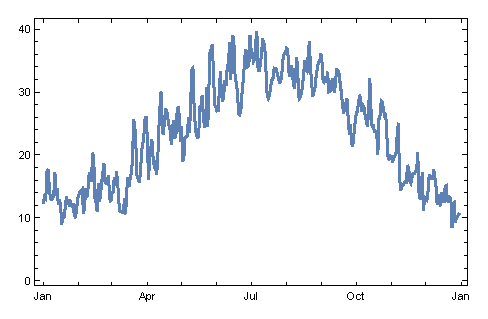
\includegraphics{GhassaneAniba_Signals_Systems_Oppenheim_Chap1_gr3.eps}

\begin{doublespace}
\noindent\(\pmb{\text{}}\)
\end{doublespace}

\begin{doublespace}
\noindent\(\pmb{\text{DiscretePlot}[\text{Prime}[n],\{n,50\}]}\)
\end{doublespace}

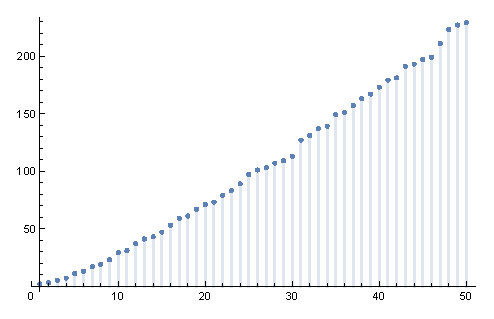
\includegraphics{GhassaneAniba_Signals_Systems_Oppenheim_Chap1_gr4.eps}

Throughout this book we will be considering two basic types of signals: continuous- time signals and discrete-time signals. In the case of continuous-time
signals the independent variable is continuous, and thus these signals are defined for a continuum of values of the independent variable. On the
other hand, discrete-time signals are defined only at discrete times, and consequently, for these signals, the independent variable takes on only
a discrete set of values. A speech signal as a function of time and atmospheric pressure as a function of altitude are examples of continuous-time
signals. The weekly Dow-Jones stock market index, as illustrated in Figure 2.6, is an example of a discrete-time signal. Other examples of discrete-time
signals can be found in demographic studies in which various attributes, such as average budget, crime rate, or pounds of fish caught, are tabulated
against such discrete variables as family size, total population, or type of fishing vessel, respectively.

\begin{doublespace}
\noindent\(\pmb{\text{Plot}[0.5*\text{Sin}[x]+2,\{x, -\text{Pi}, \text{Pi}\}, \text{PlotRange}\to \{\{-\text{Pi},\text{  }\text{Pi}\},\{0,3\}\}]}\)
\end{doublespace}

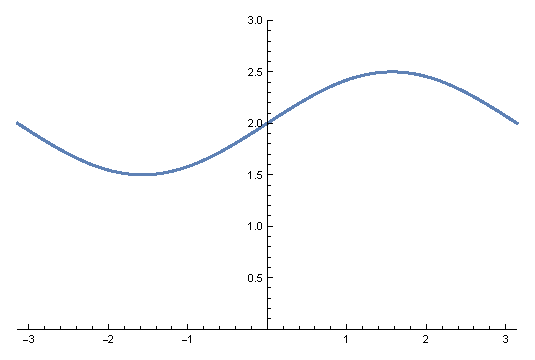
\includegraphics{GhassaneAniba_Signals_Systems_Oppenheim_Chap1_gr5.eps}

\begin{doublespace}
\noindent\(\pmb{\text{DiscretePlot}[\text{Sinc}[x],\{x, -10, 10,1\}]}\)
\end{doublespace}

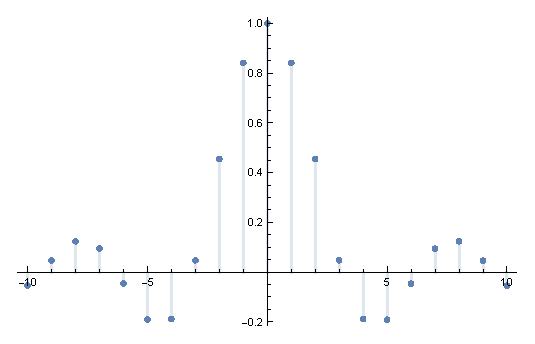
\includegraphics{GhassaneAniba_Signals_Systems_Oppenheim_Chap1_gr6.eps}

To distinguish between continuous-time and discrete-time signals, we will use the symbol \(t\) to denote the continuous-time independent variable
and \(n\) to denote the discrete-time independent variable. In addition, for continuous-time signals we will enclose the independent variable in
parentheses ($\cdot $), whereas for discrete-time signals we will use brackets [$\cdot $] to enclose the independent variable. We will also have
frequent occasions when it will be useful to represent signals graphically. Illustrations of a continuous-time signal \(x(t)\) and a discrete-time
signal \(x[n]\) are shown in Figure 2.7. It is important to note that the discrete-time signal \(x[n]\) is defined only for integer values of the
independent variable. Our choice of graphical representation for \(x[n]\) emphasizes this fact, and for further emphasis we will on occasion refer
to \(x[n]\) as a discrete-time sequence.

A discrete-time signal \(x[n\)] may represent a phenomenon for which the independent variable is inherently discrete. Signals such as demographic
data are examples of this. On the other hand, a very important class of discrete-time signals arises from the sampling of continuous-time signals.
In this case, the discrete-time signal \(x[n]\) represents successive samples of an underlying phenomenon for which the independent variable is continuous.
Because of their speed, computational power, and flexibility, modem digital processors are used to implement many practical systems, ranging from
digital autopilots to digital audio systems. Such systems require the use of discrete-time sequences representing sampled versions of continuous-time
signal - e.g., aircraft position, velocity, and heading for an autopilot or speech and music for an audio system. Also, pictures in newspapers -
or in this book, for that matter- actually consist of a very fine grid of points, and each of these points represents a sample of the brightness
of the corresponding point in the original image. No matter what the source of the data, however, the \(x[n]\) is defined only for integer values
of n. It makes no more sense to refer to the \(3\frac{1 }{2 }\)sample of a digital speech signal than it does to refer to the average budget for
a family with \(2\frac{1 }{2}\) family members.

Throughout most of this book we will treat discrete-time signals and continuous-time signals separately but in parallel, so that we can draw on insights
developed in one setting to aid our understanding of another. In Chapter 7 we will return to the question of sampling, and in that context we will
bring continuous-time and discrete-time concepts together in order to examine the relationship between a continuous-time signal and a discrete-time
signal obtained from it by sampling.

\subsection*{Signal Energy and Power}

From the range of examples provided so far, we see that signals may represent a broad variety of phenomena. In many, but not all, applications, the
signals we consider are directly related to physical quantities capturing power and energy in a physical system. For example, if v(t) and i(t) are,
respectively, the voltage and current across a resistor with resistance R, then the instantaneous power is

\begin{equation}
p(t)=v(t)i(t)=\frac{1}{R}v^2(t)
\end{equation}

The total energy expended over the time interval \(t_1\leq t\leq t_2\)is

\begin{equation}
\int_{t_1}^{t_2} p(t) \, dt=\int _{t_1}^{t_2}\frac{1}{R}v^2(t)dt,
\end{equation}

and the average power over this time interval is

\begin{equation}
\frac{1}{t_1-t_2}\int_{t_1}^{t_2} p(t) \, dt=\frac{1}{t_2-t_1}\int _{t_1}^{t_2}\frac{1}{R}v^2(t)dt
\end{equation}

Similarly, for the automobile depicted in Figure 2.2, the instantaneous power dissipated through friction is \(p(t) = b v^2(t)\), and we can then
define the total energy and average power over a time interval in the same way as in eqs. (2.2) and (2.3).

With simple physical examples such as these as motivation, it is a common and worthwhile convention to use similar terminology for power and energy
for any continuous- time signal \(x(t)\) or any discrete-time signal \(x[n]\). Moreover, as we will see shortly, we will frequently find it convenient
to consider signals that take on complex values. In this case, the total energy over the time interval \(t_1\leq t\leq t_2\) in a continuous-time
signal \(x(t)\) is defined as

\begin{equation}
\int _{t_1}^{t_2}\left|x(t)|^2dt\right.,
\end{equation}

where \(|x|\) denotes the magnitude of the (possibly complex) number \(x\). The time-averaged power is obtained by dividing eq. (2.4) by the length,
\(t_1 - t_2\), of the time interval. Similarly, the total energy in a discrete-time signal \(x[n]\) over the time interval \(n_1\leq n\leq n_2\)
is defined as

\begin{equation}
\sum _{n=n_1}^{n_2} \left|x[n]|^2\right.,
\end{equation}

and dividing by the number of points in the interval, \(n_2-n_1+1\), yields the average power over the interval. It is important to remember that
the terms {``}power{''} and {``}energy{''} are used here independently of whether the quantities in eqs. (2.4) and (2.5) actually are related to
physical energy.1 Nevertheless, we will find it convenient to use these terms ill a general fashion.

Furthermore, in many systems we will be interested in examining power and energy in signals over an infinite time interval, i.e., for \(-\infty <t<+\infty\)
or for \(-\infty <n<+\infty\). In these cases, we define the total energy as limits of eqs. (2.4) and (2.5) as the time interval increases without
bound. That is, in continuous time,

\begin{equation}
E_{\infty }\overset{\Delta }{=}\lim_{T\to  \infty } \int _{-T}^T|x(t)|^2dt=\int _{-\infty }^{+\infty }\left|x(t)|^2dt\right.,
\end{equation}

and in discrete time,

\begin{equation}
E_{\infty }\overset{\Delta }{=}\lim_{N\to \infty } \sum _{n=-N}^{+N} |x[n]|^2=\sum _{n=-\infty }^{+\infty } \left|x[n]|^2\right.,
\end{equation}

Note that for some signals the integral in eq. (2.6) or sum in eq. (2.7) might not converge- e.g., if x(t) or x[n] equals a nonzero constant value
for all time. Such signals have infinite energy, while signals with \(E_{\infty }<\infty\) have finite energy. $\cdot $

In an analogous fashion, we can define the time-averaged power over an infinite interval as

\begin{equation}
P_{\infty }\overset{\Delta }{=}\lim_{T\to \infty } \frac{1}{2T}\int _{-T}^T|x(t)|^2dt
\end{equation}

and

\begin{equation}
P_{\infty }\overset{\Delta }{=}\lim_{N\to \infty } \frac{1}{2N+1}\sum _{n=-N}^{+N} |x[n]|^2
\end{equation}

\\
in continuous time and discrete time, respectively. With these definitions, we can identify three important classes of signals. The first of these
is the class of signals with finite total energy, i.e., those signals for which \(E_{\infty }<\infty\). Such a signal must have zero average power,
since in the continuous time case, for example, we see from eq. (2.8) that

\begin{equation}
P_{\infty }=\lim_{T\to \infty } \frac{E_{\infty }}{2T}=0.
\end{equation}

An example of a finite-energy signal is a signal that takes on the value \(1\) for \(0\leq t\leq 1\) and \(0\) otherwise. In this case, \(E_{\infty
}=1\) and \(P_{\infty }=0\).

A second class of signals are those with finite average power \(P_{\infty }.\) From what we have just seen, if \(P_{\infty }>0\), then, of necessity,
\(E_{\infty }=\infty\). This, of course, makes sense, since if there is a nonzero average energy per unit time (i.e., nonzero power), then integrating
or sUmming this over an infinite time interval yields an infinite amount of energy. F9r example, the constant signal \(x[n] = 4\) has infinite energy,
but average power \(P_{\infty }=16\). There are also signals for which neither \(P_{\infty }\) nor \(E_{\infty }\) are finite. A simple example is
the signal \(x(t) = t\). We will encounter other examples of signals in each of these classes in the remainder of this and the following chapters.

\section*{NYQUIST-SHANNON SAMPLING THEOREM}

The Nyquist-Shannon Sampling theorem is a fundamental one providing the condition on the sampling frequency of a band-width limited continuous-time
signal in order to be able to reconstruct it perfectly from its discrete-time (sampled) version. It stated that the sampling frequency must be at
least two times the highest frequency of the continuous-time signal spectrum.

\subsection*{Sampling Theorem}

Sampling a continuous-time signal is getting one sample each sampling period \(T_s[s]\) , which means a sampling frequency equivalent to \(f_s=\frac{1}{T_s}[\text{Hz}]\).\\
The mean important decision to make is the sampling frequency value of \(f_s\): Indeed, if its value is too big, we{'}ll get \(f_s\) samples per
second, so large storage or large band width in order to transmit the data. If on the other hand, the value is too small, we won{'}t be able to reconstruct
the signal from the samples.\\
Hence, there is a tradeoff to make in order to minimise the needed resources (storage or frequency band-width) while being able to reproduce the
original signal from the samples.

One theorem provides an answer to this question, it{'}s the \textit{ Nyquist-Shannon Sampling Theorem} which states:

\textit{ A continuous-time signal }\textit{ \(x(t)\)}\textit{  can be sampled at a frequency }\textit{ \(f_s\)}\textit{  in order to get a discrete-time
copy of it }\textit{ \(x[n]\)}\textit{ , and afterwards be reconstructed perfectly to its original form }\textit{ \(x(t)\)}\textit{ if }\textit{
\(f_s>2f_{\max }\)}\textit{  with }\textit{ \(f_{\max }\)}\textit{  is the maximum frequency value of the }\textit{ \(x(t)\)}\textit{  signal spectrum}

Next, we{'}ll consider a \(\text{Sinc}^2\) function and see what happen to the sampled signal on the frequency domain using Fourier Transform

\subsection*{Sampling Process}

\subsubsection*{Time Domain Analysis}

Consider the function \(x(t)=\text{Sinc}^2(t)\) which represent a continuous-time signal.

Plot of the signal \(x(t)=\text{Sinc}^2(t)\):

\begin{doublespace}
\noindent\(\pmb{x[\text{t$\_$}]\text{:=}(\text{Sinc}[\text{Pi}*t]){}^{\wedge}2;}\\
\pmb{\text{Plot}[x[t],\{t,-2,2\}]}\)
\end{doublespace}

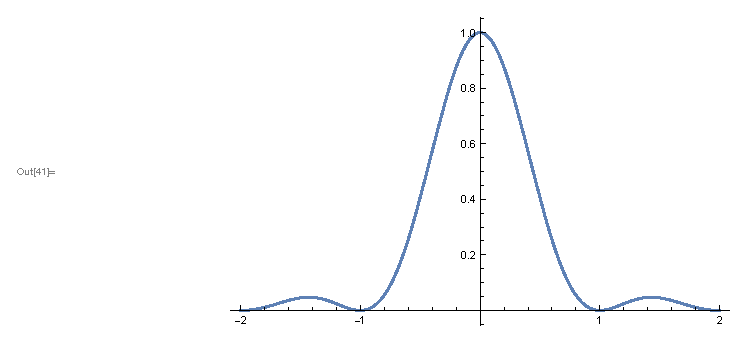
\includegraphics{GhassaneAniba_Signals_Systems_Oppenheim_Chap1_gr7.eps}

Consider a sampling frequency \(f_s\)and let see what happen for different values of \(f_s.\)

Plot of the continuous-time and discrete-time (sampled) signals:

\begin{doublespace}
\noindent\(\pmb{ \text{Manipulate}[}\\
\pmb{\text{Show}[\text{DiscretePlot}[x[t],\{t, -3, 3,1/\text{fs}\},\text{PlotRange}\to \{\{-3,3\},\{-0.1,1.1\}\},\text{PerformanceGoal}\to \text{{``}Quality{''}},\text{PlotStyle}\to
\text{Directive}[\text{Orange},\text{Thick}],\text{PlotMarkers}\to \text{Automatic}],}\\
\pmb{\text{Plot}[x[t],\{t,-3,3\}]],\{\{\text{fs},15.25,\text{{``}Frequency {''}}\}, 0.5, 30,\text{Appearance}\to \text{{``}Labeled{''}}\},\text{SaveDefinitions}\to
\text{True}]}\)
\end{doublespace}

\begin{doublespace}
\noindent\(\)
\end{doublespace}

As we can see, for high values of \(f_s\) we can at least recognize visually the original continuous-time form on the \(x(t)\) signal. However, for
small values of \(f_s\) such as \(f_s=0.1\text{hz}\) for instance, we can no more visually retrieve the form of the original \(\text{Sinc}^2\) function,
with only four sample over the 20 interval duration it{'}s quite impossible to go back from samples to continuous signal. Indeed, in such case, we
are sure not satisfying the Nyquist-Shannon sampling condition.\\
In the time domain, we can somehow visually understand what{'}s happening, however, the theorem is more understandable when analyzed on the frequency
domain.

\subsubsection*{Frequency Domain}

The spectrum analysis of signal \(x(t)\) allows us to understand easily and even prove the theorem ourselves.

\begin{equation}
\text{TF}\left[\text{Sinc}^2(a t)\right] = \frac{1}{\left| a\right| }\text{tri}\left(\frac{f}{a}\right)
\end{equation}

Fourier Transform of the signal \(x(t)\):

\begin{doublespace}
\noindent\(\pmb{\text{Simplify}[\text{FourierTransform}[x[t],t,\omega ]]}\)
\end{doublespace}

\begin{doublespace}
\noindent\(\frac{1}{4 \sqrt{2} \pi ^{3/2}}(-2 \omega  \text{Sign}[\omega ]+(-2 \pi +\omega ) \text{Sign}[-2 \pi +\omega ]+(2 \pi +\omega ) \text{Sign}[2
\pi +\omega ])\)
\end{doublespace}

Spectrum of the signal \(x(t)\):

\begin{doublespace}
\noindent\(\pmb{\text{Plot}[\text{FourierTransform}[x[t],t,\omega ],\{\omega ,-10*2 \text{Pi},10*2\text{Pi}\},\text{PlotRange}\to \{\{-2*2\text{Pi},2*2\text{Pi}\},\{0,0.41\}\}]}\)
\end{doublespace}

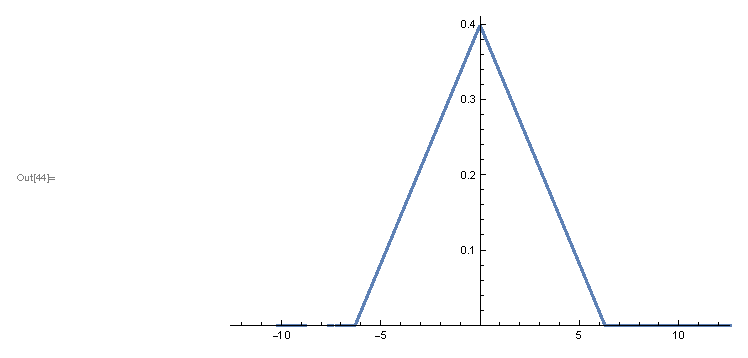
\includegraphics{GhassaneAniba_Signals_Systems_Oppenheim_Chap1_gr8.eps}

Sampled signal \(x[n]\) (left) and its Fourier transform spectrum:

\begin{doublespace}
\noindent\(\pmb{\text{Manipulate}[}\\
\pmb{\text{Row}[\{\text{DiscretePlot}[x[t],\{t, -3, 3,1/\text{fs}\},\text{PlotRange}\to \{\{-3,3\},\{-0.1,1.1\}\},\text{PerformanceGoal}\to \text{{``}Quality{''}},\text{PlotStyle}\to
\text{Directive}[\text{Orange},\text{Thick}],}\\
\pmb{\text{PlotMarkers}\to \text{Automatic},\text{ImageSize}\to 340],\text{ListLinePlot}[\text{Join}\text{@@}\text{Table}[\text{Abs}[\text{Fourier}[\text{Table}[N[x[n/\text{fs}]],\{n,-4*\text{fs},4*\text{fs}+1\}]]],4],\text{DataRange}\to
\{-4\text{Pi},4\text{Pi}\},}\\
\pmb{\text{PlotRange}\to \{\{-4\text{Pi},4\text{Pi}\},\{0,1.5\}\},\text{ImageSize}\to 300]\}],\{\{\text{fs},15.25,\text{{``}Frequency {''}}\}, 0.5,
20,\text{Appearance}\to \text{{``}Labeled{''}}\}]}\)
\end{doublespace}

\begin{doublespace}
\noindent\(\)
\end{doublespace}

The spectrum of the sampled signal is a periodic form where it{'}s period is \(2\pi\), and as long as we respect the Nyquist-Shannon condition, its
form over one period is equivalent to the spectrum of the original continuous-time signal \(x(t)\). \\
Indeed, while the sampling frequency \(f_s\)is large enough, there is no overlapping between the periods of the spectrum, and then, the original
signal can be retrieved by mean of a low passband filter. However, if the sampling frequency is too low, such as \(f_s=<\)1.4 in the above example,
there will be overlapping of the spectrum, which we call an \pmb{ \textit{ aliasing effect}}. In such a case, we can no more retrieve the original
signal using a simple low-passband filter, and we need then a more powerful signal processing by means of equalization. The condition to avoid the
overlapping is that \(f_s>2f_{\max }\), which represents perfectly the Nyquist-Shannon sampling theorem.

\textit{ * The signal looks continuous on the plot but any signal processed (transmitted, stored or displayed) is always a sampled version of the
original continuous time parameter}

\subsection*{Reconstruction Process}

The reconstruction process consists in the generation of the original continuous-time signal \(x(t)\) from the sampled version \(x[n]\). As long
as there is no aliasing effect, a simple low passband filter is enough to retrieve the original signal

Filtering the Spectrum of the sampled signal \(x[n]\):

\begin{doublespace}
\noindent\(\pmb{\text{Manipulate}[\text{Show}[\text{ListLinePlot}[\text{Join}\text{@@}\text{Table}[\text{Abs}[\text{Fourier}[\text{Table}[N[x[n/\text{fs}]],\{n,-4*\text{fs},4*\text{fs}\}]]],2],\text{DataRange}\to
\{-2\text{Pi},2\text{Pi}\},\text{PlotRange}\to \{\{-2\text{Pi},2\text{Pi}\},\{0,1.5\}\},}\\
\pmb{\text{ImageSize}\to 300],\text{Plot}[\text{HeavisidePi}[x/(2*\text{Pi})],\{x,-2\text{Pi},2\text{Pi}\},\text{Exclusions}\to \text{None},\text{PlotStyle}\to
\text{Directive}[\text{Orange},\text{Thick},\text{Dashed}] ]],}\\
\pmb{\{\{\text{fs},8,\text{{``}Frequency {''}}\}, 0.5, 20,\text{Appearance}\to \text{{``}Labeled{''}}\}]}\)
\end{doublespace}

\begin{doublespace}
\noindent\(\)
\end{doublespace}

Depending on the existence of aliasing or not, the retrieved continuous-time signal could the perfect copy of the original or a distorted one.

Spectrum of the sample signal and the reconstructed version of the signal \(x[n]\):

\begin{doublespace}
\noindent\(\pmb{\text{Manipulate}[}\\
\pmb{\text{Row}[}\\
\pmb{\{\text{Show}[\text{ListLinePlot}[\text{Join}\text{@@}\text{Table}[\text{Abs}[\text{Fourier}[\text{Table}[N[x[n/\text{fs}]],\{n,-4\text{fs},4\text{fs}\}]]],2],\text{PerformanceGoal}\to
\text{{``}Quality{''}},\text{DataRange}\to \{-2\text{Pi},2\text{Pi}\},}\\
\pmb{\text{PlotRange}\to \{\{-2\text{Pi},2\text{Pi}\},\{0,1.5\}\},\text{ImageSize}\to 300],\text{Plot}[\text{HeavisidePi}[x/(2*\text{Pi})],\{x,-2\text{Pi},2\text{Pi}\},\text{Exclusions}\to
\text{None},\text{PlotStyle}\to \text{Directive}[\text{Orange},\text{Thick},\text{Dashed}] ]],}\\
\pmb{\text{ListLinePlot}[\text{Re}[\text{InverseFourier}[\text{Fourier}[\text{Table}[N[x[n/\text{fs}]],\{n,-4\text{fs},4\text{fs}\}]]]],\text{DataRange}\to
\{-3,3\},\text{PlotRange}\to \{\{-3,3\},\{0,1.1\}\},\text{ImageSize}\to 300,}\\
\pmb{\text{PerformanceGoal}\to \text{{``}Quality{''}}] \}],\{\{\text{fs},8,\text{{``}Frequency {''}}\}, 0.5, 20,\text{Appearance}\to \text{{``}Labeled{''}}\}]}\)
\end{doublespace}

\begin{doublespace}
\noindent\(\)
\end{doublespace}

As long as the sampling frequency verifies the Nyquist-Shannon condition, we can reconstruct the original signal without distortion.

\section*{TRANSFORMATIONS OF THE INDEPENDENT VARIABLE}

A central concept in signal and system analysis is that of the transformation of a signal. For example, in an aircraft control system, signals corresponding
to the actions of the pilot are transformed by electrical and mechanical systems into changes in aircraft thrust or the positions of aircraft control
surfaces such as the rudder or ailerons, which in tum are transformed through the dynamics and kinematics of the vehicle into changes in aircraft
velocity and heading. Also, in a high-fidelity audio system, an input signal representing music as recorded on a cassette or compact disc is modified
in order to enhance desirable characteristics, to remove recording noise, or to balance the several components of the signal (e.g., treble and bass).
In this section, we focus on a very limited but important class of elementary signal transformations that involve simple modification of the independent
variable, i.e., the time axis. As we will see in this and subsequent sections of this chapter, these elementary transformations allow us to introduce
several basic properties of signals and systems. In later chapters, we will find that they also play an important role in defining and characterizing
far richer and important classes of systems.

\subsection*{Examples of Transformations of the Independent Variable}

A simple and very important example of transforming the independent variable of a signal is a time shift. A time shift in discrete time is illustrated
in Figure 2.8, in which we have two signals \(x[n]\) and \(x\left[n - n_0\right]\) that are identical in shape, but that are displaced or shifted
relative to each other. We will also encounter time shifts in continuous time, as illustrated in Figure 2.9, in which \(x\left(t - t_0\right)\) represents
a delayed (if \(t_0\)is positive) or advanced (if \(t_0\)is negative) version of x(t). Signals that are related in this fashion arise in applications
such as radar, sonar, and seismic signal processing, in which several receivers at different locations observe a signal being transmitted through
a medium (water, rock, air, etc.). In this case, the difference in propagation time from the point of origin of the transmitted signal to any two
receivers results in a time shift between the signals at the two receivers.

A second basic transformation of the time axis is that of time reversal. For example, as illustrated in Figure 2.10, the signal \(x[-n]\) is obtained
from the signal x[n] by a reflection about \(n = 0\) (i.e., by reversing the signal). Similarly, as depicted in Figure 2.11, the signal \(x(-t)\)
is obtained from the signal \(x(t)\) by a reflection about \(t = 0\). Thus, if \(x(t)\) rep- resents an audio tape recording, then \(x(- t)\) is
the same tape recording played backward. Another transformation is that of time scaling. In Figure 2.12 we have illustrated three signals, \(x(t)\),
\(x(2t)\), and \(x(t/2)\), that are related by linear scale changes in the independent variable. If we again think of the example of x(t) as a tape
recording, then \(x(2t)\) is that recording played at twice the speed, and \(x(t/2)\) is the recording played at half-speed.

It is often of interest to determine the effect of transforming the independent variable of a given signal \(x(t)\) to obtain a signal of the form
\(x(\alpha  t + \beta )\), where \(\alpha\) and \(\beta\) are given numbers. Such a transformation of the independent variable preserves the shape
of \(x(t)\), except that the resulting signal may be linearly stretched if \(|\alpha |<1\), linearly compressed if \(|\alpha |>1\) ,reversed in time
if \(\alpha <0\), and shifted in time if \(\beta\) is nonzero.This is illustrated in the following set of examples.

\begin{doublespace}
\noindent\(\pmb{\text{Original}[\text{b$\_$},\text{n$\_$},\text{d$\_$}]\text{:=}-\text{Sinc}[b*(n-d)]+5*\text{Sinc}[b*(n-d)-3];}\\
\pmb{\text{Manipulate}[\text{DiscretePlot}[\text{Original}[b,n,d], \{n, -10+d, 10+d,1\},\text{PlotRange}\to \{\{-10,10\},\{-5,5\}\},\text{PerformanceGoal}\to
\text{{``}Quality{''}}],}\\
\pmb{\{\{d,0,\text{{``}Delay{''}}\}, -5, 5,1,\text{Appearance}\to \text{{``}Labeled{''}}\},\{\{b,1,\text{{``}{''}}\},\{1\to \text{{``}Original{''}},-1\to
\text{{``}Reflected{''}}\},\text{ControlType}\to  \text{RadioButtonBar}\},\text{SaveDefinitions}\to \text{True}]}\)
\end{doublespace}

\begin{doublespace}
\noindent\(\)
\end{doublespace}

\begin{doublespace}
\noindent\(\pmb{\text{Original}[\text{b$\_$},\text{x$\_$},\text{s$\_$},\text{d$\_$}]\text{:=}-0.5*\text{Sinc}[b*(s*x-d)]+5*\text{Sinc}[b*(s*x-d)-3];}\\
\pmb{\text{Manipulate}[\text{Plot}[\text{Original}[b,x,s,d], \{x, -10, 10\},\text{PlotRange}\to \{\{-10,10\},\{-4,6\}\},\text{PerformanceGoal}\to
\text{{``}Quality{''}}],\{\{d,0,\text{{``}Delay{''}}\}, -5, 5,\text{Appearance}\to \text{{``}Labeled{''}}\},}\\
\pmb{\{\{s,1,\text{{``}Scaling{''}}\}, 0, 2,\text{Appearance}\to \text{{``}Labeled{''}}\},\{\{b,1,\text{{``}{''}}\},\{1\to \text{{``}Original{''}},-1\to
\text{{``}Reflected{''}}\},\text{ControlType}\to  \text{RadioButtonBar}\},\text{SaveDefinitions}\to \text{True}]}\)
\end{doublespace}

\begin{doublespace}
\noindent\(\)
\end{doublespace}

\subsection*{Periodic Signals}

An important class of signals that we will encounter frequently throughout this book is the class of \textit{ periodic signals}. A periodic continuous-time
signal \(x(t)\) has the property that there is a positive value of \(T\) for which

\begin{equation}
x(t)=x(t+T)
\end{equation}

for all values of \(t\). In other words, a periodic signal has the property that it is unchanged by a time shift of \(T\). In this case, we say that
\(x(t)\) is \textit{ periodic with period} \(T\) . Periodic continuous- time signals arise in a variety of contexts. For example, as illustrated
in Problem 2.61, the natural response of systems in which energy is conserved, such as ideal \textit{ LC} circuits without resistive energy dissipation
and ideal mechanical systems without frictional losses, are periodic and, in fact, are composed of some of the basic periodic signals that we will
introduce in Section 2.3.

\begin{doublespace}
\noindent\(\pmb{T=4;}\\
\pmb{g[\text{x$\_$}\text{/;}-T\leq x\leq T]\text{:=}2*\text{Sinc}[T*x];}\\
\pmb{g[\text{x$\_$}]\text{:=}g[\text{Mod}[x+T,2*T]-T];}\\
\pmb{\text{Plot}[g[x], \{x, -9*T, 9*T\},\text{PlotRange}\to \{\{-5*T,5*T\},\{-0.5,2.3\}\},\text{PerformanceGoal}\to \text{{``}Quality{''}}]}\)
\end{doublespace}

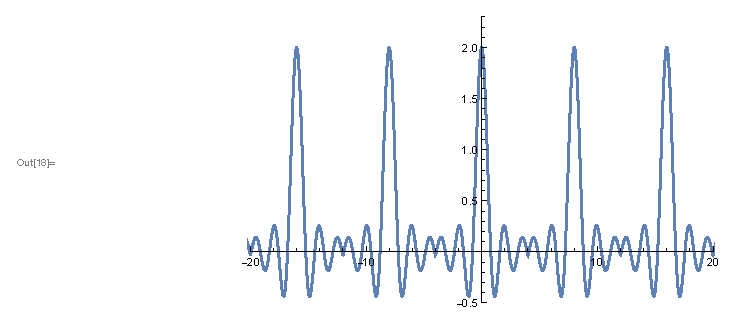
\includegraphics{GhassaneAniba_Signals_Systems_Oppenheim_Chap1_gr9.eps}

\begin{doublespace}
\noindent\(\pmb{M=4;}\\
\pmb{g[\text{n$\_$}\text{/;}-M\leq n\leq M]\text{:=}2*\text{Sinc}[M*n];}\\
\pmb{g[\text{n$\_$}]\text{:=}g[\text{Mod}[n+M,2*M]-M];}\\
\pmb{\text{DiscretePlot}[g[n], \{n, -9*M, 9*M\},\text{PlotRange}\to \{\{-5*M,5*M\},\{-0.5,2.3\}\},\text{PerformanceGoal}\to \text{{``}Quality{''}}]}\)
\end{doublespace}

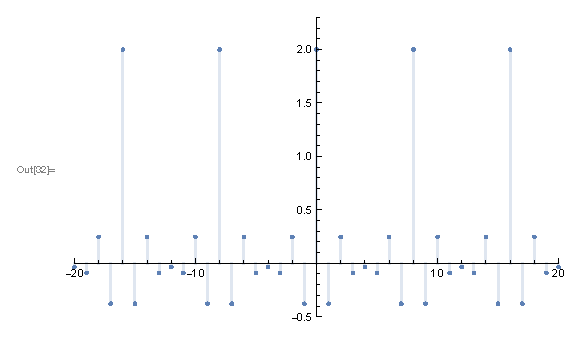
\includegraphics{GhassaneAniba_Signals_Systems_Oppenheim_Chap1_gr10.eps}

An example of a periodic continuous-time signal is given in Figure 3.3. From the figure or from eq. (3.1), we can readily deduce that if \(x(t)\)
is periodic with period \(T\), then \(x(t) = x(t + m T)\) for all t and for any integer \(m\). Thus, \(x(t)\) is also periodic with period \(2T\),
\(3T\), \(4T\), .... The \textit{ fundamental} period \(T_0\) of \(x(t)\) is the smallest positive value of \(T\) for which eq. (2.11) holds. This
definition of the fundamental period works, except if \(x(t)\) is a constant. In this case the fundamental period is undefined, since \(x(t)\) is
periodic for any choice of \(T\) (so there is no smallest positive value). A signal \(x(t)\) that is not periodic will be referred to as an aperiodic
signal.

Periodic signals are defined analogously in discrete time. Specifically, a discrete-time signal \(x[n]\) is periodic with period \(N\), where \(N\)
is a positive integer, if it is unchanged by a time shift of \(N\), i.e., if

\begin{equation}
x[n]=x[n+N]
\end{equation}

for all values of \(n\). If eq. (2.12) holds, then \(x[n]\) is also periodic with period \(2N\), \(3N\), .... The fundamental period No is the smallest
positive value of \(N\) for which eq. (l.12) holds. An example of a discrete-time periodic signal with fundamental period \(N_0 = 3\) is shown in
Figure 2.15.

\subsection*{Even and Odd Signals}

Another set of useful properties of signals relates to their symmetry under time reversal. A signal \(x(t)\) or \(x[n]\) is referred to as an even
signal if it is identical to its time-reversed counterpart, i.e., with its reflection about the origin. In continuous time a signal is even if

\begin{equation}
x(-t)=x(t)
\end{equation}

while a discrete-time signal is even if

\begin{equation}
x[-n]=x[n]
\end{equation}

A signal is referred to as odd if

\begin{equation}
x(-t)=-x(t)
\end{equation}

\begin{equation}
x[-n]=-x[n]
\end{equation}

\begin{doublespace}
\noindent\(\pmb{g[\text{x$\_$}]\text{:=}2*\text{Sinc}[T*x];\text{Plot}[g[x], \{x, -10,10\},\text{PlotRange}\to \{\{-10,10\},\{-0.5,2.3\}\},\text{PerformanceGoal}\to
\text{{``}Quality{''}}]}\)
\end{doublespace}

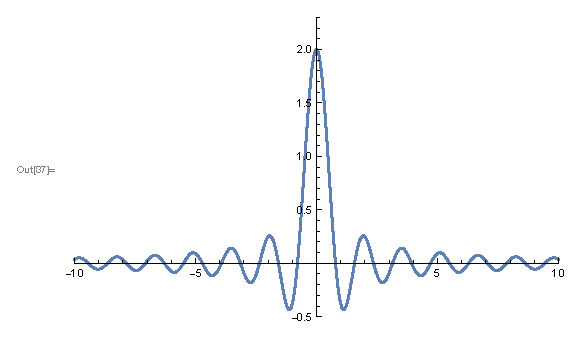
\includegraphics{GhassaneAniba_Signals_Systems_Oppenheim_Chap1_gr11.eps}

\begin{doublespace}
\noindent\(\pmb{\text{g2}[\text{x$\_$}]\text{:=}\text{Sin}[T*x];\text{Plot}[\text{g2}[x], \{x, -2,2\},\text{PlotRange}\to \{\{-2,2\},\{-1,1\}\},\text{PerformanceGoal}\to
\text{{``}Quality{''}}]}\)
\end{doublespace}

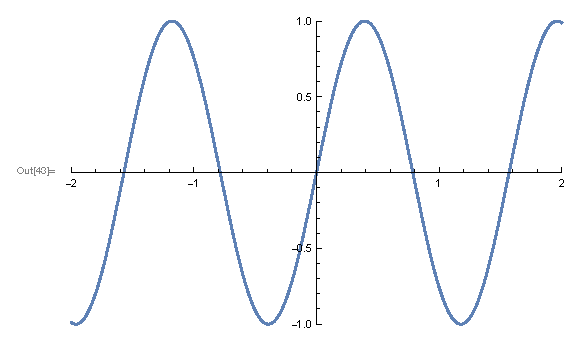
\includegraphics{GhassaneAniba_Signals_Systems_Oppenheim_Chap1_gr12.eps}

An odd signal must necessarily be \(0\) at \(t = 0\) or \(n = 0\), since eqs. (2.16) and (2.17) require that \(x(0) = - x(0)\) and \(x [0] = - x
[0]\). Examples of even and odd continuous-time signals are shown in Figure 3.17.

An important fact is that any signal can be broken into a sum of two signals, one of which is even and one of which is odd. To see this, consider
the signal

\begin{equation}
\mathcal{E}_v\{x(t)\}=\frac{1}{2}[x(t)+x(-t)]
\end{equation}

\begin{doublespace}
\noindent\(\pmb{\text{g3}[\text{n$\_$}]\text{:=}\text{Sinc}[T*(n-2)];\text{DiscretePlot}[\text{g3}[n], \{n, -10,10\},\text{PlotRange}\to \{\{-10,10\},\{-0.5,1.1\}\},\text{PerformanceGoal}\to
\text{{``}Quality{''}}]}\)
\end{doublespace}

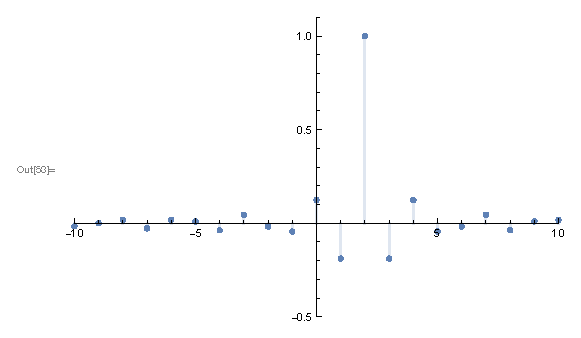
\includegraphics{GhassaneAniba_Signals_Systems_Oppenheim_Chap1_gr13.eps}

\begin{doublespace}
\noindent\(\pmb{\text{g4}[\text{n$\_$}]\text{:=}(\text{g3}[n]+\text{g3}[-n])/2;}\\
\pmb{\text{DiscretePlot}[\text{g4}[n], \{n, -10,10\},\text{PlotRange}\to \{\{-10,10\},\{-0.2,0.6\}\},\text{PerformanceGoal}\to \text{{``}Quality{''}}]}\)
\end{doublespace}

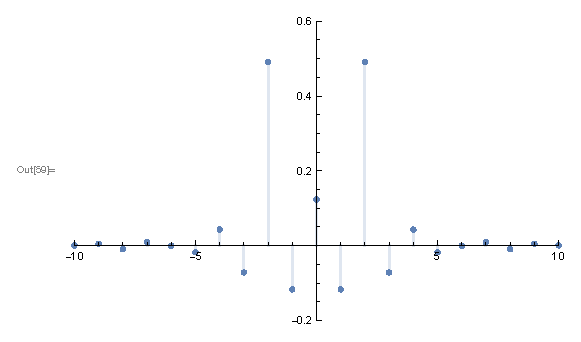
\includegraphics{GhassaneAniba_Signals_Systems_Oppenheim_Chap1_gr14.eps}

which is referred to as the even part of x(t). Similarly, the odd part of x(t) is given by

\begin{equation}
\mathcal{O}\mathit{d}\{x(t)\}=\frac{1}{2}[x(t)-x(-t)]
\end{equation}

\begin{doublespace}
\noindent\(\pmb{\text{g4}[\text{n$\_$}]\text{:=}(\text{g3}[n]-\text{g3}[-n])/2;}\\
\pmb{\text{DiscretePlot}[\text{g4}[n], \{n, -10,10\},\text{PlotRange}\to \{\{-10,10\},\{-0.6,0.6\}\},\text{PerformanceGoal}\to \text{{``}Quality{''}}]}\)
\end{doublespace}

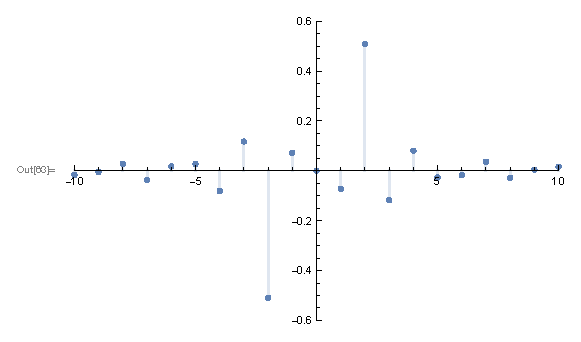
\includegraphics{GhassaneAniba_Signals_Systems_Oppenheim_Chap1_gr15.eps}

It is a simple exercise to check that the even part is in fact even, that the odd part is odd, and that \(x(t)\) is the sum of the two. Exactly analogous
definitions hold in the discrete- time case. An example of the even-odd decomposition of a discrete-time signal is given in Figure 1.18.

\section*{EXPONENTIAL AND SINUSOIDAL SIGNALS}

In this section and the next, we introduce several basic continuous-time and discrete-time signals. Not only do these signals occur frequently, but
they also serve as basic building blocks from which we can construct many other signals.

\subsection*{Continuous-Time Complex Exponential and Sinusoidal Signals}

The continuous-time complex exponential signal is of the form

\begin{equation}
x(t)=A e^{a t}
\end{equation}

where \(C\) and \(a\) are, in general, complex numbers. Depending upon the values of these parameters, the complex exponential can exhibit several
different characteristics.

\pmb{ Real Exponential Signals}

As illustrated in Figure 1.19, if \(C\) and \(a\) are real [in which case \(x(t)\) is called a real exponential], there are basically two types of
behavior. If \(a\) is positive, then as \(t\) increases \(x(t)\) is a growing exponential, a form that is used in describing many different physical
processes, including chain reactions in atomic explosions and complex chemical reactions. If \(a\) is negative, then \(x(t)\) is a decaying exponential,
a signal that is also used to describe a wide variety of phenomena, including the process of radioactive decay and the responses of \textit{ RC}
circuits and damped mechanical systems. In particular, as shown in Problems 1.61 and 1.62, the natural responses of the circuit in Figure 1.1 and
the automobile in Figure 1.2 are decaying exponentials. Also, we note that for \(a = 0\), \(x(t)\) is constant.

\begin{doublespace}
\noindent\(\pmb{\text{Original1}[\text{b$\_$},\text{A$\_$},\text{x$\_$}]\text{:=}A*\text{Exp}[b*x];}\\
\pmb{\text{Manipulate}[\text{Plot}[\text{Original1}[g*b,A,x], \{x, -10, 10\},\text{PlotRange}\to \{\{-10,10\},\{0,4\}\},\text{PerformanceGoal}\to
\text{{``}Quality{''}},}\\
\pmb{\text{Epilog}\to \{\{\text{Text}[\text{Style}[\text{A},\text{Black},\text{Bold},12],\{-1,A\}]\},\{\text{Line}[\{\{-0.5,A\},\{+0.5,A\}\}]\}\}],\{\{b,0.3,\text{{``}Exponent{''}}\},
0, 1,\text{Appearance}\to \text{{``}Labeled{''}}\},}\\
\pmb{\{\{A,1,\text{{``}Coeff{''}}\}, 0, 2,\text{Appearance}\to \text{{``}Labeled{''}}\},\{\{g,1,\text{{``}{''}}\},\{1\to \text{{``}Original{''}},-1\to
\text{{``}Reflected{''}}\}\},\text{SaveDefinitions}\to \text{True}]}\)
\end{doublespace}

\begin{doublespace}
\noindent\(\pmb{}\)
\end{doublespace}

\pmb{ Periodic Complex Exponential and Sinusoidal Signals}

A second important class of complex exponentials is obtained by constraining a to be purely imaginary. Specifically, consider

\begin{equation}
x(t)=C e^{\text{j$\omega $}_0t}
\end{equation}

An important property of this signal is that it is periodic. To verify this, we recall from eq. (1.11) that \(x(t)\) will be periodic with period
\(T\) if

\begin{equation}
e^{\text{j$\omega $}_0t}=e^{\text{j$\omega $}_0(t+T)}
\end{equation}

\\
Or, since

\begin{equation}
e^{\text{j$\omega $}_0t}=e^{\text{j$\omega $}_0t}e^{\text{j$\omega $}_0T}
\end{equation}

it follows that for periodicity, we must have

\begin{equation}
e^{\text{j$\omega $}_0T}=2.
\end{equation}

If \(\omega _0 = 0\), then \(x(t) = 1\), which is periodic for any value of \(T\). If \(\omega _0\neq 0\), then the fundamental period To of x(t)
- that is, the smallest positive value of \(T_0\) for which eq. (l.23) holds - is

\begin{equation}
T_0=\frac{2\pi }{\left|\omega _0\right|}.
\end{equation}

Thus, the signals \(e^{\text{j$\omega $}_0t}\) and \(e^{-\text{j$\omega $}_0t}\) have the same fundamental period.\\
A signal closely related to the periodic complex exponential is the sinusoidal signal

\begin{equation}
x(t)=A \cos \left(\omega _0t+\phi \right),
\end{equation}

as illustrated in Figure 1.20. With seconds as the units of \(t\), the units of $\phi $ and \(\omega _0\) are radians and radians per second, respectively.
It is also common to write \(\omega _0=2\pi  f_0\).where \(f_0\)has the units of cycles per second, or hertz (Hz). Like the complex exponential signal,
the sinusoidal signal is periodic with fundamental period \(T_0\) given by eq. (1.24). Sinusoidal and complex exponential signals are also used to
describe the characteristics of many physical processes-in particular, physical systems in which energy is conserved. For example, as shown in Problem
1.61, the natural response of an \textit{ LC} circuit is sinusoidal, as is the simple harmonic motion of a mechanical system consisting of a mass
connected by a spring to a stationary support. The acoustic pressure variations corresponding to a single musical tone are also sinusoidal.

\begin{doublespace}
\noindent\(\pmb{\text{Manipulate}[\text{Plot}[a*\text{Cos}[2*\text{Pi}*f*t + \text{phi}], \{t, -20, 20\},\text{PlotRange}\to \{\{-5,15\},\{-5,5\}\},\text{PerformanceGoal}\to
\text{{``}Quality{''}},}\\
\pmb{\text{Epilog}\to \left\{\left\{\text{Text}\left[\text{Style}\left[\text{$\texttt{"}$T=}\frac{2\pi }{\omega _0}\texttt{"},\text{Black},\text{Bold},12\right],\{-\text{phi}/(2*\text{Pi}*f)+1/(2*f),a+0.2\}\right]\right\},\{\text{Text}[\text{Style}[\text{{``}A.Cos($\phi
$){''}},\text{Black},\text{Bold},12],\{-2.8,a*\text{Cos}[\text{phi}]\}]\},\right.}\\
\pmb{\{\text{Line}[\{\{-\text{phi}/(2*\text{Pi}*f),a-0.3\},\{-\text{phi}/(2*\text{Pi}*f),a+0.5\}\}]\},\{\text{Line}[\{\{-\text{phi}/(2*\text{Pi}*f)+1/f,a-0.3\},\{-\text{phi}/(2*\text{Pi}*f)+1/f,a+0.5\}\}]\},}\\
\pmb{\{\text{Arrow}[\{\{-\text{phi}/(2*\text{Pi}*f)+3/(8*f)-0.5,a+0.3\},\{-\text{phi}/(2*\text{Pi}*f),a+0.3\}\}]\},\{\text{Arrow}[\{\{-\text{phi}/(2*\text{Pi}*f)+5/(8*f)+0.5,a+0.3\},\{-\text{phi}/(2*\text{Pi}*f)+1/f,a+0.3\}\}]\},}\\
\pmb{\{\text{Line}[\{\{-0.3,a*\text{Cos}[\text{phi}]\},\{+0.3,a*\text{Cos}[\text{phi}]\}\}]\}\}],\{\{a,3,\text{{``}Amplitude{''}}\}, 0, 5,\text{Appearance}\to
\text{{``}Labeled{''}}\},\{\{f,0.15,\text{{``}Frequency{''}}\}, 0.001, 0.7,\text{Appearance}\to \text{{``}Labeled{''}}\},}\\
\pmb{\{\{\text{phi},-1,\text{{``}Delay{''}}\}, -10, 10,\text{Appearance}\to \text{{``}Labeled{''}}\},\text{SaveDefinitions}\to \text{True}]}\)
\end{doublespace}

\begin{doublespace}
\noindent\(\pmb{}\)
\end{doublespace}

\begin{doublespace}
\noindent\(\pmb{\text{Manipulate}[\text{DiscretePlot}[a*\text{Cos}[2*\text{Pi}*f*(n - p)], \{n, 0, 40\},\text{PlotRange}\to \{\{0,40\},\{-5,5\}\},\text{PerformanceGoal}\to
\text{{``}Quality{''}}],}\\
\pmb{\{\{a,3,\text{{``}Amplitude{''}}\}, 0.1, 5,\text{Appearance}\to \text{{``}Labeled{''}}\},\{\{f,0.2,\text{{``}Frequency{''}}\}, 0.1, 10,\text{Appearance}\to
\text{{``}Labeled{''}}\},\{\{p,0,\text{{``}Delay{''}}\}, 0, 10,1,\text{Appearance}\to \text{{``}Labeled{''}}\},}\\
\pmb{\text{SaveDefinitions}\to \text{True}]}\)
\end{doublespace}

\begin{doublespace}
\noindent\(\)
\end{doublespace}

By using Euler's relation, the complex exponential in eq. (l.21) can be written in terms of sinusoidal signals with the same fundamental period:

\begin{equation}
e^{\text{j$\omega $t}}=\cos  \omega _0t+j \text{sin$\omega $}_0t.
\end{equation}

Similarly, the sinusoidal signal of eq. (1.25) can be written in terms of periodic complex\\
exponentials, again with the same fundamental period:

\begin{equation}
\text{Acos}\left(\omega _0t+\phi \right)=\frac{A}{2}e^{\text{j$\phi $}}e^{\text{j$\omega $}_0t}+\frac{A}{2}e^{-\text{j$\phi $}}e^{-\text{j$\omega
$}_0t}
\end{equation}

Note that the two exponentials in eq. (1.27) have complex amplitudes. Alternatively, we can express a sinusoid in terms of a complex exponential
signal as

\begin{equation}
\text{Acos}\left(\omega _0t+\phi \right)=\text{$\mathcal{R}$e}\left\{\frac{A}{2}e^{\left(\text{j$\omega $}_0t+\phi \right)}\right\}
\end{equation}

where, if c is a complex number, $\mathcal{R}$e$\{$c$\}$ denotes its real part. We will also use the notation $\mathcal{I}$m$\{$c$\}$ for the imaginary
part of c, so that, for example,

\begin{equation}
\text{Asin}\left(\omega _0t+\phi \right)=\text{A$\mathcal{I}$m}\left\{\frac{A}{2}e^{\left(\text{j$\omega $}_0t+\phi \right)}\right\}
\end{equation}

From eq. (1.24), we see that the fundamental period \(T_0\) of a continuous-time sinusoidal signal or a periodic complex exponential is inversely
proportional to \(\left\left| \omega _0\right.\)$\right| $ which we will refer to as the fundamental frequency. From Figure 1.21, we see graphically
what this means. If we decrease the magnitude of \(\omega _0\), we slow down the rate of oscillation and therefore increase the period. Exactly the
opposite effects occur if we increase the magnitude of \(\omega _0\). Consider now the case \(\omega _0=0\). In this case, as we mentioned earlier,
\(x(t)\) is constant and therefore is periodic with period \(T\) for any positive value of \(T\). Thus, the fundamental period of a constant signal
is undefined. On the other hand, there is no ambiguity in defining the fundamental frequency of a constant signal to be zero. That is, a constant
signal has a zero rate of oscillation.

Periodic sig\\
nals-and in particular, the complex periodic exponential signal in eq. (1.21) and the sinusoidal signal in eq.( 1.25) - provide important examples
of signals with infinite total energy but finite average power. For example, consider the periodic exponential signal of eq. (l.21), and suppose
that we calculate the total energy and average power in this signal over one period:

\begin{doublespace}
\noindent\(\pmb{\text{}}\)
\end{doublespace}

Since there are an infinite number of periods as t ranges from -oo to +oo, the total energy integrated over all time is infinite. However, each period
of the signal looks exactly the same. Since the average power of the signal equals 1 over each period, averaging over multiple periods always yields
an average power of 2. That is, the complex periodic exponential signal has finite average power equal to



Problem 1.3 provides additional examples of energy and power calculations for periodic and aperiodic signals. $\cdot $\\
Periodic complex exponentials will play a central role in much of our treatment of signals and systems, in part because they serve as extremely useful
building blocks for many other signals. We will often find it useful to consider sets of harmonically related complex exponentials-that is, sets
of periodic exponentials, all of which are periodic with a common period T0$\bullet $ Specifically, a necessary condition for a complex exponential
ejwt to be periodic with period To is that

\begin{equation}
\text{}
\end{equation}

which implies that wT0 is a multiple of 27T, i.e.,



Thus, if we define



we see that, to satisfy eq. (1.34), w must be an integer multiple of wo. That is, a harmonically related set of complex exponentials is a set of
periodic exponentials with fundamental frequencies that are all multiples of a single positive frequency w 0 :



Fork = 0, $<$f$>$k(t) is a constant, while for any other value of k, $<$f$>$k(t) is periodic with fundamental frequency Iklwo and fundamental period



The kth harmonic $<$f$>$k(t) is still periodic with period To as well, as it goes through exactly lkl of its fundamental periods during any time
interval of length T0 $\bullet $

Our use of the term {``}harmonic{''} is consistent with its use in music, where it refers to tones resulting from variations in acoustic pressure
at frequencies that are integer multiples of a fundamental frequency. For example, the pattern of vibrations of a string on an instrument such as
a violin can be described as a superposition-i.e., a weighted sum-of harmonically related periodic exponentials. In Chapter 3, we will see that we
can build a very rich class of periodic signals using the harmonically related signals of eq. (1.36) as the building blocks.

General Complex Exponential Signals

The most general case of a complex exponential can be expressed and interpreted in terms of the two cases we have examined so far: the real exponential
and the periodic complex exponential. Specifically, consider a complex exponential Ceat, where C is expressed in polar form and a in rectangular
form. That is,



and



Then



Using Euler{'}s relation, we can expand this further as



Thus, for r = 0, the real and imaginary parts of a complex exponential are sinusoidal. For r $>$ 0 they correspond to sinusoidal signals multiplied
by a growing exponential, and for r $<$ 0 they correspond to sinusoidal signals multiplied by a decaying exponential. These two cases are shown in
Figure 1.23. The dashed lines in the figure correspond to the functions $\pm $ICJer1$\bullet $ From eq. (l.42), we see that ICJer1 is the magnitude
of the complex expo- nential: Thus, the dashed curves act as an envelope for the oscillatory curve in the figure in that the peaks of the oscillations
just reach these curves, and in this way the envelope provides us with a convenient way to visualize the general trend in the amplitude of the oscillations.



Sinusoidal signals multiplied by decaying exponentials are commonly referred to as daniped sinusoids. Examples of damped sinusoids arise in the response
of RLC circuits and in mechanical systems containing both damping and restoring forces, such as automotive suspension systems. These kinds of systems
have mechanisms that dissipate energy (resistors, damping forces such as friction) with oscillations that decay in time. Examples illustrating such
systems and their damped sinusoidal natural responses can be found in Problems 1.61 and 1.62.

\subsection*{Discrete-Time Complex Exponential and Sinusoidal Signals}

As in continuous time, an important signal in discrete time is the complex exponential signal or sequence, defined by



where C and a are, in general, complex numbers. This could alternatively be expressed in the form



Although the form of the discrete-time complex exponential sequence given in eq. (1.45) is more analogous to the form of the continuous-time exponential,
it is often more convenient to express the discrete-time complex exponential sequence in the form of eq. (l.44).



Real Exponential Signals

If C and a are real, we can have one of several types of behavior, as illustrated in Figure 1.24.Iflal $>$ 1 the magnitude of the signal grows exponentially
with n, while if l a l $<$ 1 we have a decaying exponential. Furthermore, if a is positive, all the values of Ca{''} are of the same sign, but if
a is negative then the sign of x[n] alternates. Note also that if a = 1 then x[n] is a constant, whereas if a = -1, x[n] alternates in value between
+C and - C. Real-valued discrete-time exponentials are often used to describe population growth as a function of generation and total return on investment
as a function of day, month, or quarter.

Sinusoidal Signals

Another important complex exponential is obtained by using the form given in eq. (1.45) and by constraining $\{$3 to be purely imaginary (so that
lal = 1). Specifically, consider



As in the continuous-time case, this signal is closely related to the sinusoidal sign



If we take n to be dimensionless, thenbothw0 and $<$/$>$ have units of radians.Three examples of sinusoidal sequences are shown in Figure 1.25.\\
As before, Euler's relation allows us to relate complex exponentials and sinusoids:



and



The signals in eqs. (1.46) and (l.47) are examples of discrete-time signals with infinite total energy but finite average power. For example, since
lejwonl2 = 1, every sample of the signal in eq. (1.46) contributes 1 to the signal{'}s energy. Thus, .the total energy for -oo $<$ n $<$ oo is infinite,
while the average power per time point is obviously equal to 2. Other examples of energy and power calculations for discrete-time signals are given
in Problem 1.3.



General Complex Exponential Signals

The general discrete-time complex exponential can be written and interpreted in terms of real exponentials and sinusoidal signals. Specifically,
if we write C and a in polar form,









Thus, for lal = 1, the real and imaginary parts of a complex exponential sequence are sinusoidal. For laI$<$ 1 tliey correspond to sinusoidal sequences
multiplied by a decaying exponential, while for lal $>$ 1 they correspond to sinusoidal sequences multiplied by a growing exponential. Examples of
these signals are depicted in Figure 1.26.

\subsection*{Periodicity Properties of Discrete-Time Complex Exponentials}

While there are many similarities between continuous-time and discrete-time signals, there are also a number of important differences. One of these
concerns the discrete-time exponential signal ejwon . In Section 3.3.1, we identified the following two properties of its continuous-time counterpart
ejwot: (1)thelargerthemagnitudeofw0, the higher is the rate of oscillation in the signal; and (2) ej{''}{'}o1 is periodic for any value ofw0$\bullet
$ In this section we de.scribe the discrete-time versions of both of these properties, and as we will see, there are definite differences between
each of these and its continuous-time counterpart.\\
The fact that the first of these properties is different in discrete time is a direct consequence of another extremely important distinction between
discrete-time and continuous- time complex exponentials. Specifically, consider the discrete-time complex exponential with frequency wo + 27T:





From eq. (3.51), we see that the exponential at frequency w0 + 27T is the same as that at frequency w 0 . Thus, we have a very different situation
from the continuous-time case, in which the signals ejwot are all distinct for distinct values of w 0 . In discrete time, these signals are not distinct,
as the signal with frequency w0 is identical to the signals with frequencies wo $\pm $ 27T, wo $\pm $ 47T, and so on. Therefore, in considering discrete-time
com- plex exponentials, we need only consider a frequency interval of length 27T in which to choose wo. Although, according to eq. (3.51), any interval
of length 27T will do, on most occasions we will use the interval 0 :s w0 $<$ 27T or the interval -7T :s w 0 $<$ 1T .\\
Because of the periodicity implied by eq. (3.51), the signal ejwon does not have a continually increasing rate of oscillation as w0 is increased
in magnitude. Rather, as il- lustrated in Figure 1.27, as we increase w0 from 0, we obtain signals that oscillate more and more rapidly until we
reach wo = 1T. As we continue to increase wo, we decrease the rate of oscillation until we reach wo = 27T, which produces the same constant sequence
as w0 = 0. Therefore, the low-frequency (that is, slowly varying) discrete-time exponentials have values of wo near 0, 27T, and any other even multiple
of 7T, while the high frequencies (corresponding to rapid variations) are located near w 0 = $\pm $ 1T and other odd multiples of 7T. Note in particular
that for w0 = 1T or any other odd multiple of 7T,



\\
so that this signal oscillates rapidly, changing sign at each point in time [as illustrated in Figure 1.27(e)].\\
The second property we wish to consider concerns the periodicity of the discrete- time complex exponential. In order for the signal ejwon to be periodic
with period N $>$ 0, we must have



or equivalently,



For eq. (1.54) to hold, woN must be a multiple of 2$\pi $. That is, there must be an integer m such that



or equivalently,



According to eq. (l.56), the signal eiwon is periodic if wo/27T is a rational number and is not periodic otherwise. These same observations also
hold for discrete-time sinusoids. For example, the signals depicted in Figure l.25(a) and (b) are periodic, while the signal in Figure l.25(c) is
not.\\
Using the calculations that we have just made, we can also determine the funda- mental period and frequency of discrete-time complex exponentials,
where we define the fundamental frequency of a discrete-time periodic signal as we did in continuous time. That is, if x[n] is periodic with fundamental
periodN, its fundamental frequency is 27T/N. Consider, then, a periodic complex exponential x[n] = eiwon with w0 $\#$ 0. As we have just seen, w0
must satisfy eq. (1.56) for some pair of integers m and N, with N $>$ 0. In Problem 1.35, it is shown that if wo $\#$ 0 and if N and m have no factors
in common, then the fundamental period of x[n] is N. Using this fact together with eq. (1.56), we find that the fundamental frequency of the periodic
signal { }is



Note that the fundamental period can also be written as



These last two expressions again differ from their continuous-time counterparts. In Table 1.1, we have summarized some of the differences between
the continuous-time signal eiwot and the discrete-time signal eiwon. Note that, as in the continuous-time case, the constant discrete-time signal
resulting from setting wo = 0 has a fundamental frequency of zero, and its fundamental period is undefined.



\\
To gain some additional insight into these properties, let us examine again the signals depicted in Figure 1.25. First, consider the sequence x[n]
= cos(2$\pi $n/12), depicted in Figure 1.25(a), which we can think of as the set of samples of the continuous-time sinusoid x(t) = cos(2$\pi $t/12)
at integer time points. In this case, x(t) is periodic with fundamental period 12 and x [n] is also periodic with fundamental period 12. That is,
the values of x [n] repeat every 12 points, exactly in step with the fundamental period of x(t).

In contrast, consider the signal x[n] = cos(87Tn/31), depicted in Figure 1.25(b), which we can view as the set of samples of x(t) = cos (87Tt/31)
at integer points in time. In this case, x(t) is periodic with fundamental period 3114. On the other hand, x[n] is periodic with fundamental period
32. The reason for this difference is that the discrete-time signal is defined only for integer values of the independent variable. Thus, there is
no sample at time t = 3114, when x(t) completes one period (starting from t = 0). Similarly, there is no sample at t = 2$\cdot $31/4ort = 3$\cdot
$31/4, when x(t) has completed two or three periods, but there is a sample at t = 4 $\cdot $ 3114 = 31, when x(t) has completed four periods. This
can be seen in Figure 1.25(b), where the pattern of x[n] values does not repeat with each single cycle of positive and negative values. Rather, the
pattern repeats after four such cycles, namely, every 31 points.

Similarly, the signal x[n] = cos(n/6) can be viewed as the set of samples of the signal x(t) = cos(t/6) at integer time points. In this case, the
values of x(t) at integer sample points never repeat, as these sample points never span an interval that is an exact multiple of the period, 127T,
of x(t). Thus, x[n] is not periodic, although the eye visually interpolates between the sample points, $\cdot $suggesting the envelope x(t), which
is periodic. The use of the concept of sampling to gain insight into the periodicity of discrete-time sinusoidal sequences is explored further in
Problem 1.36.

\(\text{Example}\)

Suppose that we wish to determine the fundamental period of the discrete-time signal. \\
The first exponential on the right-hand side of eq. (1.59) has a fundamental period of 3. While this can be verified from eq. (1.58), there is a
simpler way to obtain that answer. In particular, note that the angle (27r/3)n of the first term must be incremented by a multiple of 27r for the
values of this exponential to begin repeating. We then immediately see that if n is incremented by 3, the angle will be incremented by a single multiple
of 27r. With regard to the second term, we see that incrementing the angle (37r/4)n by 27r would require n to be incremented by 8/3, which is impossible,
since n is restricted to being an integer. Similarly, incrementing the angle by 47r would require a noninteger increment of 16/3 ton. However, incrementing
the angle by 67r requires an increment of 8 ton, and thus the fundamental period of the second term is 8.\\
Now, for the entire signal x[n] to repeat, each of the terms in eq. (l.59) must go through an integer number of its own fundamental period. The smallest
increment of n that accomplishes this is 24. That is, over an interval of 24 points, the first term on the right-hand side of eq. (1 .59) will have
gone through eight of its fundamental periods, the second term through three of its fundamental periods, and the overall signal x[n] through exactly
one of its fundamental periods.

As in continuous time, it is also of considerable value in discrete-time signal and system analysis to consider sets of harmonically related periodic
exponentials-that is, periodic exponentials with a common period N. From eq. (l.56), we know that these are precisely the signals which are at frequencies
which are multiples of 27T/N. That is,



In the { }continuous-time case, all of the harmonically related complex exponentials { } 2, ..., are distinct. However, because of eq. (1.51), this
is not the case in discrete time. Specifically,



This implies that there are only N distinct periodic exponentials in the set given in eq. (1 .60). For example,



are all distinct, and any other $<$f$>$k[n] is identical to one of these (e.g., $<$f$>$N[n] = $<$Po[n] and $<$P- 1[n] = $<$P- 1[n]).

\section*{THE UNIT IMPULSE AND UNIT STEP FUNCTIONS}

In this section, we introduce several other basic signals-specifically, the unit impulse and step functions in continuous and discrete time-that
are also of considerable importance in signal and system analysis. In Chapter 2, we will see how we can use unit impulse signals as basic building
blocks for the construction and representation of other signals. We begin with the discrete-time case.

\subsection*{The Continuous-Time Unit Step and Unit Impulse Functions}

The continuous-time unit step function u(t) is defined in a manner similar to its discrete-time counterpart. Specifically,



as is shown in Figure 1.32. Note that the unit step is discontinuous at t = 0. The continuous-time unit impulse function 8(t) is related to the unit
step in a manner analogous to the relationship between the discrete-time unit impulse and step functions. In particular, the continuous-time unit
step is the running integral of the unit impulse



This also suggests a relationship between li(t) and u(t) analogous to the expression for li[n] in eq. (l.65). In particular, it follows from eq.
(1.71) that the continuous-time unit impulse can be thought of as the first derivative of the continuous-time unit step:



In contrast to the discrete-time case, there is some formal difficulty with this equation as a representation of the unit impulse function, since
u(t) is discontinuous at t = 0 and consequently is formally not differentiable. We can, however, interpret eq. (1.72) by considering an approximation
to the unit step Ufl(t), as illustrated in Figure 1.33, which rises from the value 0 to the value 1 in a short time interval of length .::l. The
unit step, of course, changes values instantaneously and thus can be thought of as an idealization of Ufl(t) for Ll so short that its duration doesn{'}t
matter for any practical purpose. Formally, u(t) is the limit of { } { } { }as $\Delta $ { } 0. Let us now consider the derivative



as shown in Figure 1.34.



Note that 8!l(t) is a short pulse, of { } { } { } { } { } and with unit area for any value { } { } { } { } { } { }0,8!l(t) becomes narrower and higher,
maintaining its unit area. Its limiting form,



can then be thought of as an idealization of the short pulse 8!l(t) as the duration becomes insignificant. Since 8(t) has, in effect, no duration
but unit area, we adopt the graphical notation for it shown in Figure 1.35, where the arrow at t =0 indicates that the area of the pulse is concentrated
at t = 0 and the height of the arrow and the {``}1{''} next to the arrow are used to represent the area of the impulse. More generally, a scaled
impulse k8(t) will have an area k, and thus,

 

A scaled impulse with area k is shown in Figure 1.36, where the height of the arrow used to depict the scaled impulse is chosen to be proportional
to the area of the impulse.

As with discrete time, we can provide a simple graphical interpretation of the running integral of eq. (l.71); this is shown in Figure 1.37. Since
the area of the continuous-time unit impulse 8(r) is concentrated at T = 0, we see that the running integral is 0 for t $<$ 0 and 1 fort $>$ 0. Also,
we note that the relationship in eq. (1.71) between the continuous- time unit step and impulse can be rewritten in a different form, analogous to
the discrete- time form in eq. (l.67), by changing the variable of integration from T to $<$r = t - r:



or equivalently,



The graphical interpretation of this form of the relationship between u(t) and 8(t) is given in Figure 1.38. Since in this case the area of 8(t -
$<$r) is concentrated at the point $<$r = t, we again see that the integral in eq. (l.75) is 0 fort $<$ 0 and 1 fort $>$ 0. This type of graphical
interpretation of the behavior of the unit impulse under integration will be extremely useful in Chapter 2.





As with the discrete-time impulse, the continuous-time impulse has a very important sampling property. In particular, for a number of reasons it
will be important to consider the product of an impulse and more well-behaved continuous-time functions x(t). The interpretation of this quantity
is most readily developed using the definition of 8(t) according to eq. (l.74). Specifically, consider



In Figure l.39(a) we have depicted the two time functions x(t) and 8il(t), and in Figure l.39(b) we see an enlarged view of the nonzero portion of
their product. By construction x 1(t) is zero outside the interval 0 :s t :s A. For A sufficiently small so that x(t) is approximately constant over
this interval,



Since 8(t) is the limit as A { } 0 of 8ii(t), it follows that



By the same argument, we have an analogous expression for an impulse concentrated at an arbitrary point, say, t0 . That is,



Although our discussion of the unit impulse in this section has been somewhat in- formal, it does provide us with some important intuition about
this signal that will be useful throughout the book. As we have stated, the unit impulse should be viewed as an idealization. As we illustrate and
discuss in more detail in Section 1.5, any real physical system has some inertia associated with it and thus does not respond instantaneously to
inputs. Consequently, if a pulse of sufficiently short duration is applied to such a system, the system response will not be noticeably influenced
by the pulse{'}s duration or by the details of the shape of the pulse, for that matter. Instead, the primary characteristic of the pulse that will
matter is the net, integrated effect of the pulse-Le., its area. For systems that respond much more quickly than others, the pulse will have to be
of much shorter duration before the details of the pulse shape or its duration no longer matter. Nevertheless, for any physical system, we can always
find a pulse that is {``}short enough.{''} The unit impulse then is an idealization of this concept-the pulse that is short enough for any system.
As we will see in Chapter 2, the response of a system to this idealized pulse plays a crucial role in signal and system analysis, and in the process
of developing and understanding this role, we will develop additional insight into the idealized signal.

Example 1.7

Consider the discontinuous signal x(t) depicted in Figure l.40(a). Because of the relationship between the continuous-time unit impulse and unit
step, we can readily calculate and graph the derivative of this signal. Specifically, the derivative of x(t) is clearly 0, except at the discontinuities.
In the case of the unit step, we have seen [eq. (1.72)] that differentiation gives rise to a unit impulse located at the point of discontinuity.
Further- more, by multiplying both sides of eq. (1.72) by any number k, we see that the derivative of a unit step with a discontinuity of size k
gives rise to an impulse of area k at the point of discontinuity. This rule also holds for any other signal with a jump discontinuity, such as x(t)
in Figure l.40(a). Consequently, we can sketch its derivative x(t), as in Figure 1.40(b), where an impulse is placed at each discontinuity of x(t),
with area equal to the size of the discontinuity. Note, for example, that the discontinuity in x(t) at t = 2 has a value of -3, so that an impulse
scaled by -3 is located at t= 2 in the signal x(t).

As a check of our result, we can verify that we can recover x(t) from i(t). Specifically, since x(t) and i(t) are both zero for { } { } ,we need
only check that fort $>$ 0,



As illustrated in Figure l.40(c), fort$<$ 1, the integral on the right-hand side of eq. (1.77) is zero, since none of the impulses that constitute
i(t) are within the interval of integration. For 1 $<$ t $<$ 2, the first impulse (located at t = 1) is the only one within the integration interval,
and thus the integral in eq. (1.77) equals 2, the area of this impulse. For 2 $<$ t $<$ 4, the first two impulses are within the interval of integration,
and the integral accumulates the sum of both of their areas, namely, 2 - 3 = -1 . Finally, for t $>$ 4, all three impulses are within the integration
interval, so that the integral equals the sum of all three areas-that is, 2 - 3 + 2 = +2. The result is exactly the signal x(t) depicted in Figure
l.40(a).

\section*{CONTINUOUS-TIME AND DISCRETE-TIME SYSTEMS}

Physical systems in the broadest sense are an interconnection of components, devices, or subsystems. In contexts ranging from signal processing and
communications to electromechanical motors, automotive vehicles, and chemical-processing plants, a system can be viewed as a process in which input
signals are transformed by the system or cause the system to respond in some way, resulting in other signals as outputs. For example, a high-fidelity
system takes a recorded audio signal and generates a reproduction of that signal. If the hi-fi system has tone controls, we can change the tonal
quality of the reproduced signal. Similarly, the circuit in Figure 1.1 can be viewed as a system with input voltage V5 (t) and output voltage Vc(t),
while the automobile in Figure 1.2 can be thought of as a system with input equal to the force f(t) and output equal to the velocity v(t) of the
vehicle. An image-enhancement system transforms an input image into an output image that has some desired properties, such as improved contrast.

A continuous-time system is a system in which continuous-time input signals are applied and result in continuous-time output signals. Such a system
will be represented pictorially as in Figure l.41(a), where x(t) is the input and y(t) is the output. Alternatively, we will often represent the
input-output relation of a continuous-time system by the notation

Similarly, a discrete-time system-that is, a system that transforms discrete-time inputs into discrete-time outputs-will be depicted as in Figure
l.4l(b) and will sometimes be represented symbolically as



In most of this book, we will$\cdot $treat discrete-time systems and continuous-time systems separately but in parallel. In Chapter 7, we will bring
continuous-time and discrete-time systems together through the concept of sampling, and we will develop some insights into the use of discrete-time
systems to process continuous-time signals that have been sampled.

\subsection*{Simple Examples of Systems}

One of the most important motivations for the development of general tools for analyzing and designing systems is that systems from many different
applications have very similar mathematical descriptions. To illustrate this, we begin with a few simple examples.

Example 1.8

Consider the RC circuit depicted in Figure 1.1. If we regard v,(t) as the input signal and vc(t) as the output signal, then we can use simple circuit
analysis to derive an equation describing the relationship between the input and output. Specifically, from Ohm{'}s law, the current i(t) through
the resistor is proportional (with proportionality constant 1/R) to the voltage drop across the resistor; i.e.,



Similarly, using the defining constitutive relation for a capacitor, we can relate i(t) to the rate of change with time of the voltage across the
capacitor:



Equating the right-hand sides of eqs. (1.80) and (1.81), we obtain a differential equation describing the relationship between the input v,(t) and
the output vc(t):

Example 1.9

Example 1.10

Example 1.11

As the preceding examples suggest, the mathematical descriptions of systems from a wide variety of applications frequently have a great deal in common,
and it is this fact that provides considerable motivation for the development of broadly applicable tools for signal and system analysis. The key
to doing this successfully is identifying classes of systems that have two important characteristics: (1) The systems in this class have properties
and structures that we can exploit to gain insight into their behavior and to develop effective tools for their analysis; and (2) many systems of
practical importance can be accurately modeled using systems in this class. It is on the first of these characteristics that most of this book focuses,
as we develop tools for a particular class of systems referred to as linear, time-invariant systems. In the next section, we will introduce the properties
that characterize this class, as well as a number of other very important basic system properties.

The second characteristic mentioned in the preceding paragraph is of obvious importance for any system analysis technique to be of value in practice.
It is a well-established fact that a wide range of physical systems (including those in Examples 1.8- 1.10) can be well modeled within the class
of systems on which we focus in this book. However, a critical point is that any model used in describing or analyzing a physical system rep- resents
an idealization of that system, and thus, any resulting analysis is only as good as the model itself. For example, the simple linear model of a resistor
in eq. (1.80) and that of a capacitor in eq. (l.81) are idealizations. However, these idealizations are quite accurate for real resistors and capacitors
in many applications, and thus, analyses employing such idealizations provide useful results and conclusions, as long as the voltages and currents
remain within the operating conditions under which these simple linear models are valid. Similarly, the use of a linear retarding force to represent
frictional effects in eq. (l.83) is an approximation with a range of validity. Consequently, although we will not address this issue in the book,
it is important to remember that an essential component of engineering practice in using the methods we develop here consists of identifying the
range of validity of the assumptions that have gone into a model and ensuring that any analysis or design based on that model does not violate those
assumptions.

\subsection*{Interconnections of Systems}

An important idea that we will use throughout this book is the concept of the interconnection of systems. Many real systems are built as interconnections
of several subsystems. One example is an audio system, which involves the interconnection of a radio receiver, compact disc player, or tape deck
with an amplifier and one or more speakers. Another is a digitally controlled aircraft, which is an interconnection of the aircraft, described by
its equations of motion and the aerodynamic forces affecting it; the sensors, which measure various aircraft variables such as accelerations, rotation
rates, and heading; a digital autopilot, which responds to the measured variables and to command inputs from the pilot (e.g., the desired course,
altitude, and speed); and the aircraft{'}s actuators, which respond to inputs provided by the autopilot in order to use the aircraft control surfaces
(rudder, tail, ailerons) to change the aerodynamic forces on the aircraft. By viewing such a system as an interconnection of its components, we can
use our understanding of the component systems and of how they are interconnected in order to analyze the operation and behavior of the overall system.
In addition, by describing a system in terms of an interconnection of simpler subsystems, we may in fact be able to define useful ways in which to
synthesize complex systems out of simpler, basic building blocks.

While one can construct a variety of system interconnections, there are several basic ones that are frequently encountered. A series or cascade interconnection
of two systems is illustrated in Figure l.42(a). Diagrams such as this are referred to as block diagrams. Here, the output of System 1 is the input
to System 2, and the overall system transforms an input by processing it first by System 1 and then by System 2. An example of a series interconnection
is a radio receiver followed by an amplifier. Similarly, one can define a series interconnection of three or more systems.

A parallel interconnection of two systems is illustrated in Figure l.42(b). Here, the same input signal is applied to Systems 1 and 2. The symbol
{``}EB{''} in the figure denotes addition, so that the output of the parallel interconnection is the sum of the outputs of Systems 1 and 2. An example
of a parallel interconnection is a simple audio system with several microphones feeding into a single amplifier and speaker system. In addition to
the simple parallel interconnection in Figure 1.42(b), we can define parallel interconnections of more than two systems, and we can combine both
cascade and parallel interconnections to obtain more complicated interconnections. An example of such an interconnection is given in Figure l.42(c).

Another important type of system interconnection is a feedback interconnection, an example of which is illustrated in Figure 1.43. Here, the output
of System 1 is the input to System 2, while the output of System 2 is fed back and added to the external input to produce the actual input to System
2. Feedback systems arise in a wide variety of applications. For example, a cruise control system on an automobile senses the vehicle's velocity
and adjusts the fuel flow in order to keep the speed at the desired level. Similarly, a digitally controlled aircraft is most naturally thought of
as a feedback system in which differences between actual and desired speed, heading, or altitude are fed back through the autopilot in order to correct
these discrepancies. Also, electrical circuits are often usefully viewed as containing feedback interconnections. As an example, consider the circuit
depicted in Figure l.44(a). As indicated in Figure l.44(b), this system can be viewed as the feedback interconnection of the two circuit elements.

\begin{doublespace}
\noindent\(\pmb{\text{Nyquist}-\text{Shannon} \text{Sampling} \text{Theorem}}\\
\pmb{\text{The} \text{Nyquist}-\text{Shannon} \text{Sampling} \text{theorem} \text{is} a \text{fundamental} \text{one} \text{providing} \text{the}
\text{condition} \text{on} \text{the} \text{sampling} \text{frequency} \text{of} a \text{band}-}\\
\pmb{\text{width} \text{limited} \text{continuous}-\text{time} \text{signal} \text{in} \text{order} \text{to} \text{be} \text{able} \text{to} \text{reconstruct}
\text{it} \text{perfectly} \text{from} \text{its} \text{discrete}-}\\
\pmb{\text{time} (\text{sampled}) \text{version}.\text{It} \text{stated} \text{that} \text{the} \text{sampling} \text{frequency} \text{must} \text{be}
\text{at} \text{least} \text{two} \text{times} \text{the} \text{highest} \text{frequency} \text{of} \text{the} \text{continuous}-}\\
\pmb{\text{time} \text{signal} \text{spectrum}.}\\
\pmb{\text{What} \text{is} a \text{Signal}?}\\
\pmb{A \text{signal} \text{is} a \text{time}/\text{space} \text{varying} \text{function} \text{which} \text{includes} \text{some} \text{useful} \text{information}.\text{Most}
\text{of} \text{signals} \text{are} \text{continuous}-}\\
\pmb{\text{time} \text{ones} \text{and} \text{hence} \text{can} \text{not} \text{be} \text{either} \text{stored} (\text{or} \text{transmitted}) \text{over}
\text{realistic} \text{limited} \text{data} \text{storage} (\text{or} \text{band}-\text{limited} \text{propagation} \text{space}) }\\
\pmb{\text{due} \text{to} \text{infinity} \text{of} \text{points} \text{to} \text{be} \text{processed}.\text{Such} \text{signals} \text{could} \text{be}
\text{of} \text{different} \text{sources} \text{or} \text{types},\text{such} \text{as} \text{audio} }\\
\pmb{\text{ones},\text{or} \text{any} \text{real} \text{life} \text{physical} \text{measure} \text{or} \text{parameter} \text{retrieved} \text{by}
\text{sensors} (\text{temp},\text{humidity},\text{speed},\text{...}).}\\
\pmb{\text{Example} \text{of} a \text{continuous}-\text{time}*\text{signal}-\text{Mean} \text{Temperature} \text{during} 2016 \text{in} \text{Rabat},\text{Morocco}:}\\
\pmb{\text{weatherData}=\text{WeatherData}[\{33.9716,6.8498\}, \text{{``}MeanTemperature{''}}, \{\{2016, 1, 1\}, \{2016, 12, 31\}, \text{{``}Day{''}}\}];}\\
\pmb{\text{DateListPlot}[\text{weatherData},\text{Joined} \text{-$>$} \text{True}]}\\
\pmb{}\\
\pmb{\text{In} \text{order},\text{to} \text{process} \text{real} \text{life} \text{signals} \text{either} \text{to} \text{store} \text{or} \text{transmit},\text{we}
\text{need} \text{to} a\pmb{\text{\textit{sampling}}}\pmb{\text{\textit{$ $}}}\pmb{\text{\textit{process}}}\text{them},\text{making} \text{them}\pmb{\text{\textit{discrete}}}\pmb{\text{\textit{$-$}}}\pmb{\text{\textit{time}}}\pmb{\text{\textit{$
$}}}\pmb{\text{\textit{signal}}}.}\\
\pmb{\text{Sampling} \text{Theorem}}\\
\pmb{\text{Sampling} a \text{continuous}-\text{time} \text{signal} \text{is} \text{getting} \text{one} \text{sample} \text{each} \text{sampling}
\text{period} ,\text{which} \text{means} a \text{sampling} \text{frequency} }\\
\pmb{\text{equivalent} \text{to}.\text{The} \text{mean} \text{important} \text{decision} \text{to} \text{make} \text{is} \text{the} \text{sampling}
\text{frequency} \text{value} \text{of}:\text{Indeed},\text{if} \text{its} \text{value} \text{is} \text{too} \text{big},\text{we}\text{'}}\\
\pmb{\text{ll} \text{get}\text{samples} \text{per} \text{second},\text{so} \text{large} \text{storage} \text{or} \text{large} \text{band} \text{width}
\text{in} \text{order} \text{to} \text{transmit} \text{the} \text{data}.\text{If} \text{on} \text{the} \text{other} \text{hand},\text{the} \text{value}
\text{is} \text{too} \text{small},\text{we} \text{won}\text{'}}\\
\pmb{t \text{be} \text{able} \text{to} \text{reconstruct} \text{the} \text{signal} \text{from} \text{the} \text{samples}.\text{Hence},\text{there}
\text{is} a \text{tradeoff} \text{to} \text{make} \text{in} \text{order} \text{to} \text{minimise} \text{the} \text{needed} \text{resources} }\\
\pmb{(\text{storage} \text{or} \text{frequency} \text{band}-\text{width}) \text{while} \text{being} \text{able} \text{to} \text{reproduce} \text{the}
\text{original} \text{signal} \text{from} \text{the} \text{samples}.}\\
\pmb{\text{One} \text{theorem} \text{provides} \text{an} \text{answer} \text{to} \text{this} \text{question},\text{it}\text{'}s \text{the}\text{\textit{Nyquist}}\text{\textit{$-$}}\text{\textit{Shannon}}\text{\textit{$
$}}\text{\textit{Sampling}}\text{\textit{$ $}}\text{\textit{Theorem}}\text{which} \text{states}:}\\
\pmb{\text{\textit{$A \text{continuous}$}}\text{\textit{$-$}}\text{\textit{time}}\text{\textit{$ $}}\text{\textit{signal}}\text{\textit{$ $}}\text{\textit{$
$}}\text{\textit{can}}\text{\textit{$ $}}\text{\textit{be}}\text{\textit{$ $}}\text{\textit{sampled}}\text{\textit{$ $}}\text{\textit{at}}\text{\textit{$
$}}\text{\textit{$a$}}\text{\textit{$ $}}\text{\textit{frequency}}\text{\textit{$ $}}\text{\textit{$ $}}\text{\textit{in}}\text{\textit{$ $}}\text{\textit{order}}\text{\textit{$
$}}\text{\textit{to}}\text{\textit{$ $}}\text{\textit{get}}\text{\textit{$ $}}\text{\textit{$a$}}\text{\textit{$ $}}\text{\textit{discrete}}\text{\textit{$-$}}\text{\textit{time}}\text{\textit{$
$}}\text{\textit{copy}}\text{\textit{$ $}}\text{\textit{of}}\text{\textit{$ $}}\text{\textit{it}}\text{\textit{$ $}}\text{\textit{$,$}}\text{\textit{$
$}}}\\
\pmb{\text{\textit{and}}\text{\textit{$ $}}\text{\textit{afterwards}}\text{\textit{$ $}}\text{\textit{be}}\text{\textit{$ $}}\text{\textit{reconstructed}}\text{\textit{$
$}}\text{\textit{perfectly}}\text{\textit{$ $}}\text{\textit{to}}\text{\textit{$ $}}\text{\textit{its}}\text{\textit{$ $}}\text{\textit{original}}\text{\textit{$
$}}\text{\textit{form}}\text{\textit{$ $}}\text{\textit{if}}\text{\textit{$ $}}\text{\textit{$ $}}\text{\textit{with}}\text{\textit{$ $}}\text{\textit{$
$}}\text{\textit{is}}\text{\textit{$ $}}\text{\textit{the}}\text{\textit{$ $}}\text{\textit{maximum}}\text{\textit{$ $}}\text{\textit{frequency}}\text{\textit{$
$}}\text{\textit{value}}\text{\textit{$ $}}\text{\textit{of}}\text{\textit{$ $}}\text{\textit{the}}\text{\textit{$ $}}\text{\textit{$ $}}\text{\textit{signal}}\text{\textit{$
$}}\text{\textit{spectrum}}}\\
\pmb{\text{Next},\text{we}\text{'}\text{ll} \text{consider} a\text{function} \text{and} \text{see} \text{what} \text{happen} \text{to} \text{the}
\text{sampled} \text{signal} \text{on} \text{the} \text{frequency} \text{domain} \text{using} \text{Fourier} \text{Transform}}\\
\pmb{\text{Sampling} \text{Process}}\\
\pmb{\text{Time} \text{Domain} \text{Analysis}}\\
\pmb{\text{Consider} \text{the} \text{function}\text{which} \text{represent} a \text{continuous}-\text{time} \text{signal}.}\\
\pmb{\text{Plot} \text{of} \text{the} \text{signal}:}\\
\pmb{x[\text{t$\_$}]\text{:=}(\text{Sinc}[\text{Pi}*t]){}^{\wedge}2;}\\
\pmb{\text{Plot}[x[t],\{t,-2,2\}]}\\
\pmb{}\\
\pmb{\text{Consider} a \text{sampling} \text{frequency}\text{and} \text{let} \text{see} \text{what} \text{happen} \text{for} \text{different} \text{values}
\text{of}}\\
\pmb{\text{Plot} \text{of} \text{the} \text{continuous}-\text{time} \text{and} \text{discrete}-\text{time} (\text{sampled}) \text{signals}:}\\
\pmb{ \text{Manipulate}[}\\
\pmb{\text{Show}[\text{DiscretePlot}[x[t],\{t, -3, 3,1/\text{fs}\},\text{PlotRange}\to \{\{-3,3\},\{-0.1,1.1\}\},\text{PerformanceGoal}\to \text{{``}Quality{''}},\text{PlotStyle}\to
\text{Directive}[\text{Orange},\text{Thick}],}\\
\pmb{\text{PlotMarkers}\to \text{Automatic}],\text{Plot}[x[t],\{t,-3,3\}]],}\\
\pmb{\{\{\text{fs},15.25,}\\
\pmb{\text{{``}Frequency $\unicode{f7c1}\unicode{f7c9}\unicode{f7c8}$Cell[TextData[Cell[BoxData[$\backslash $nFormBox[$\backslash $nSubscriptBox[$\backslash
${''}f$\backslash ${``}, $\backslash ${''}s$\backslash \texttt{"}$], }}\\
\pmb{\text{TraditionalForm]],ExpressionUUID-$>\backslash ${``}a9724fa4-f400-4ac7-a61f-924698fc7ada$\backslash ${''}]],ExpressionUUID-$>\backslash
\texttt{"}$471a2222-e15d-}}\\
\pmb{\text{416c-ad54-06bebb600fe2$\backslash ${``}]$\unicode{f7c0}${''}}\}, 0.5, 30,\text{Appearance}\to \text{{``}Labeled{''}}\},}\\
\pmb{\text{SaveDefinitions}\to \text{True}]}\\
\pmb{}\\
\pmb{\text{As} \text{we} \text{can} \text{see},\text{for} \text{high} \text{values} \text{of}\text{we} \text{can} \text{at} \text{least} \text{recognize}
\text{visually} \text{the} \text{original} \text{continuous}-\text{time} \text{form} \text{on} \text{the}\text{signal}.\text{However},}\\
\pmb{\text{for} \text{small} \text{values} \text{of}\text{such} \text{as}\text{for} \text{instance},\text{we} \text{can} \text{no} \text{more} \text{visually}
\text{retrieve} \text{the} \text{form} \text{of} \text{the} \text{original}\text{function},}\\
\pmb{\text{with} \text{only} \text{four} \text{sample} \text{over} \text{the} 20 \text{interval} \text{duration} \text{it}\text{'}s \text{quite}
\text{impossible} \text{to} \text{go} \text{back} \text{from} \text{samples} \text{to} \text{continuous} \text{signal}.\text{Indeed},\text{in} \text{such}
\text{case},}\\
\pmb{\text{we} \text{are} \text{sure} \text{not} \text{satisfying} \text{the} \text{Nyquist}-\text{Shannon} \text{sampling} \text{condition}.\text{In}
\text{the} \text{time} \text{domain},\text{we} \text{can} \text{somehow} \text{visually} \text{understand} \text{what}\text{'}s \text{happening},}\\
\pmb{\text{however},\text{the} \text{theorem} \text{is} \text{more} \text{understandable} \text{when} \text{analyzed} \text{on} \text{the} \text{frequency}
\text{domain}.}\\
\pmb{\text{Frequency} \text{Domain}}\\
\pmb{\text{The} \text{spectrum} \text{analysis} \text{of} \text{signal}\text{allows} \text{us} \text{to} \text{understand} \text{easily} \text{and}
\text{even} \text{prove} \text{the} \text{theorem} \text{ourselves}.}\\
\pmb{}\\
\pmb{\text{Fourier} \text{Transform} \text{of} \text{the} \text{signal}:}\\
\pmb{\text{Simplify}[\text{FourierTransform}[x[t],t,\omega ]]}\\
\pmb{\frac{1}{4 \sqrt{2} \pi ^{3/2}}(-2 \omega  \text{Sign}[\omega ]+(-2 \pi +\omega ) \text{Sign}[-2 \pi +\omega ]+(2 \pi +\omega ) \text{Sign}[2
\pi +\omega ])}\\
\pmb{\text{Spectrum} \text{of} \text{the} \text{signal}:}\\
\pmb{\text{Plot}[\text{FourierTransform}[x[t],t,\omega ],\{\omega ,-10*2 \text{Pi},10*2\text{Pi}\},\text{PlotRange}\to \{\{-2*2\text{Pi},2*2\text{Pi}\},\{0,0.41\}\}]}\\
\pmb{}\\
\pmb{\text{Sampled} \text{signal}(\text{left}) \text{and} \text{its} \text{Fourier} \text{transform} \text{spectrum}:}\\
\pmb{\text{Manipulate}[}\\
\pmb{\text{Row}[\{\text{DiscretePlot}[x[t],\{t, -3, 3,1/\text{fs}\},\text{PlotRange}\to \{\{-3,3\},\{-0.1,1.1\}\},\text{PerformanceGoal}\to \text{{``}Quality{''}},\text{PlotStyle}\to
\text{Directive}[\text{Orange},\text{Thick}],}\\
\pmb{\text{PlotMarkers}\to \text{Automatic},\text{ImageSize}\to 340],\text{ListLinePlot}[\text{Join}\text{@@}\text{Table}[\text{Abs}[\text{Fourier}[\text{Table}[N[x[n/\text{fs}]],\{n,-4*\text{fs},4*\text{fs}+1\}]]],4],}\\
\pmb{\text{DataRange}\to \{-4\text{Pi},4\text{Pi}\},\text{PlotRange}\to \{\{-4\text{Pi},4\text{Pi}\},\{0,1.5\}\},\text{ImageSize}\to 300]\}],}\\
\pmb{\{\{\text{fs},15.25,}\\
\pmb{\text{{``}Frequency $\unicode{f7c1}\unicode{f7c9}\unicode{f7c8}$Cell[TextData[Cell[BoxData[$\backslash $nFormBox[$\backslash $nSubscriptBox[$\backslash
${''}f$\backslash ${``}, $\backslash ${''}s$\backslash \texttt{"}$], }}\\
\pmb{\text{TraditionalForm]],ExpressionUUID-$>\backslash ${``}a2cb0041-6aef-4f93-ae3e-c4d0221b8fe1$\backslash ${''}]],ExpressionUUID-$>\backslash
\texttt{"}$1ddeba3a-2146-414c-b45b-}}\\
\pmb{\text{df60412b7ea1$\backslash ${``}]$\unicode{f7c0}${''}}\}, 0.5, 20,\text{Appearance}\to \text{{``}Labeled{''}}\}]}\\
\pmb{}\\
\pmb{\text{The} \text{spectrum} \text{of} \text{the} \text{sampled} \text{signal} \text{is} a \text{periodic} \text{form} \text{where} \text{it}\text{'}s
\text{period} \text{is},\text{and} \text{as} \text{long} \text{as} \text{we} \text{respect} \text{the} \text{Nyquist}-\text{Shannon} \text{condition},}\\
\pmb{\text{its} \text{form} \text{over} \text{one} \text{period} \text{is} \text{equivalent} \text{to} \text{the} \text{spectrum} \text{of} \text{the}
\text{original} \text{continuous}-\text{time} \text{signal}.\text{Indeed},\text{while} \text{the} \text{sampling} \text{frequency}\text{is} \text{large}
\text{enough},}\\
\pmb{\text{there} \text{is} \text{no} \text{overlapping} \text{between} \text{the} \text{periods} \text{of} \text{the} \text{spectrum},\text{and}
\text{then},\text{the} \text{original} \text{signal} \text{can} \text{be} \text{retrieved} \text{by} \text{mean} \text{of} a \text{low} \text{passband}
\text{filter}.\text{However},}\\
\pmb{\text{if} \text{the} \text{sampling} \text{frequency} \text{is} \text{too} \text{low},\text{such} \text{as}1.4 \text{in} \text{the} \text{above}
\text{example},\text{there} \text{will} \text{be} \text{overlapping} \text{of} \text{the} \text{spectrum},\text{which} \text{we} \text{call} \text{an}\pmb{\text{\textit{aliasing}}}\pmb{\text{\textit{$
$}}}\pmb{\text{\textit{effect}}}.\text{In} \text{such} a \text{case},}\\
\pmb{\text{we} \text{can} \text{no} \text{more} \text{retrieve} \text{the} \text{original} \text{signal} \text{using} a \text{simple} \text{low}-\text{passband}
\text{filter},}\\
\pmb{\text{and} \text{we} \text{need} \text{then} a \text{more} \text{powerful} \text{signal} \text{processing} \text{by} \text{means} \text{of}
\text{equalization}.\text{The} \text{condition} \text{to} \text{avoid} \text{the} \text{overlapping} \text{is} \text{that},}\\
\pmb{\text{which} \text{represents} \text{perfectly} \text{the} \text{Nyquist}-\text{Shannon} \text{sampling} \text{theorem}.}\\
\pmb{\text{\textit{$* \text{The} \text{signal} \text{looks} \text{continuous} \text{on} \text{the} \text{plot} \text{but} \text{any} \text{signal}
\text{processed} (\text{transmitted}, \text{stored} \text{or} \text{displayed}) \text{is} \text{always} a \text{sampled} \text{version} \text{of}
\text{the} \text{original} \text{continuous} \text{time} \text{parameter}$}}}\\
\pmb{\text{Reconstruction} \text{Process}}\\
\pmb{\text{The} \text{reconstruction} \text{process} \text{consists} \text{in} \text{the} \text{generation} \text{of} \text{the} \text{original}
\text{continuous}-\text{time} \text{signal}\text{from} \text{the} \text{sampled} \text{version}.\text{As} \text{long} \text{as} \text{there} \text{is}
\text{no} \text{aliasing} \text{effect},}\\
\pmb{a \text{simple} \text{low} \text{passband} \text{filter} \text{is} \text{enough} \text{to} \text{retrieve} \text{the} \text{original} \text{signal}}\\
\pmb{\text{Filtering} \text{the} \text{Spectrum} \text{of} \text{the} \text{sampled} \text{signal}:}\\
\pmb{\text{Manipulate}[\text{Show}[\text{ListLinePlot}[\text{Join}\text{@@}\text{Table}[\text{Abs}[\text{Fourier}[\text{Table}[N[x[n/\text{fs}]],\{n,-4*\text{fs},4*\text{fs}\}]]],2],\text{DataRange}\to
\{-2\text{Pi},2\text{Pi}\},\text{PlotRange}\to \{\{-2\text{Pi},2\text{Pi}\},\{0,1.5\}\},}\\
\pmb{\text{ImageSize}\to 300],\text{Plot}[\text{HeavisidePi}[x/(2*\text{Pi})],\{x,-2\text{Pi},2\text{Pi}\},\text{Exclusions}\to \text{None},\text{PlotStyle}\to
\text{Directive}[\text{Orange},\text{Thick},\text{Dashed}] ]],}\\
\pmb{\{\{\text{fs},8,}\\
\pmb{\text{{``}Frequency $\unicode{f7c1}\unicode{f7c9}\unicode{f7c8}$Cell[TextData[Cell[BoxData[$\backslash $nFormBox[$\backslash $nSubscriptBox[$\backslash
${''}f$\backslash ${``}, $\backslash ${''}s$\backslash \texttt{"}$], }}\\
\pmb{\text{TraditionalForm]],ExpressionUUID-$>\backslash ${``}5fb84079-c017-47ed-b2bb-190f843e1bb1$\backslash ${''}]],ExpressionUUID-$>\backslash
${``}2301db58-70f8-4ced-a0f4-d37ce295ffb0$\backslash ${''}]$\unicode{f7c0}\texttt{"}$}\}, }\\
\pmb{0.5, 20,\text{Appearance}\to \text{{``}Labeled{''}}\}]}\\
\pmb{}\\
\pmb{\text{Depending} \text{on} \text{the} \text{existence} \text{of} \text{aliasing} \text{or} \text{not},\text{the} \text{retrieved} \text{continuous}-\text{time}
\text{signal} \text{could} \text{the} \text{perfect} \text{copy} \text{of} \text{the} \text{original} \text{or} a \text{distorted} \text{one}.}\\
\pmb{\text{Spectrum} \text{of} \text{the} \text{sample} \text{signal} \text{and} \text{the} \text{reconstructed} \text{version} \text{of} \text{the}
\text{signal}:}\\
\pmb{\text{Manipulate}[}\\
\pmb{\text{Row}[}\\
\pmb{\{\text{Show}[\text{ListLinePlot}[\text{Join}\text{@@}\text{Table}[\text{Abs}[\text{Fourier}[\text{Table}[N[x[n/\text{fs}]],\{n,-4\text{fs},4\text{fs}\}]]],2],\text{PerformanceGoal}\to
\text{{``}Quality{''}},\text{DataRange}\to \{-2\text{Pi},2\text{Pi}\},}\\
\pmb{\text{PlotRange}\to \{\{-2\text{Pi},2\text{Pi}\},\{0,1.5\}\},\text{ImageSize}\to 300],\text{Plot}[\text{HeavisidePi}[x/(2*\text{Pi})],\{x,-2\text{Pi},2\text{Pi}\},\text{Exclusions}\to
\text{None},}\\
\pmb{\text{PlotStyle}\to \text{Directive}[\text{Orange},\text{Thick},\text{Dashed}] ]],}\\
\pmb{\text{ListLinePlot}[\text{Re}[\text{InverseFourier}[\text{Fourier}[\text{Table}[N[x[n/\text{fs}]],\{n,-4\text{fs},4\text{fs}\}]]]],\text{DataRange}\to
\{-3,3\},\text{PlotRange}\to \{\{-3,3\},\{0,1.1\}\},\text{ImageSize}\to 300,}\\
\pmb{\text{PerformanceGoal}\to \text{{``}Quality{''}}] \}],}\\
\pmb{\{\{\text{fs},8,}\\
\pmb{\text{{``}Frequency $\unicode{f7c1}\unicode{f7c9}\unicode{f7c8}$Cell[TextData[Cell[BoxData[$\backslash $nFormBox[$\backslash $nSubscriptBox[$\backslash
${''}f$\backslash ${``}, $\backslash ${''}s$\backslash \texttt{"}$], }}\\
\pmb{\text{TraditionalForm]],ExpressionUUID-$>\backslash ${``}321d93b0-2af2-470e-8995-ba7ea2807a8d$\backslash ${''}]],ExpressionUUID-$>\backslash
${``}91dddb38-0015-4fff-ae4b-d00ba63cd2c3$\backslash ${''}]$\unicode{f7c0}\texttt{"}$}\},}\\
\pmb{ 0.5, 20,\text{Appearance}\to \text{{``}Labeled{''}}\}]}\\
\pmb{}\\
\pmb{\text{As} \text{long} \text{as} \text{the} \text{sampling} \text{frequency} \text{verifies} \text{the} \text{Nyquist}-\text{Shannon} \text{condition},\text{we}
\text{can} \text{reconstruct} \text{the} \text{original} \text{signal} \text{without} \text{distortion}.}\\
\pmb{\text{Further} \text{Explorations}}\\
\pmb{\text{Digital} \text{Signal} \text{Processing}}\\
\pmb{\text{Analog} \text{and} \text{Digital} \text{Modulation} \text{Techniques}}\\
\pmb{\text{Authorship} \text{information}}\\
\pmb{\text{Ghassane} \text{Aniba}}\\
\pmb{23 \text{June} 2017}\\
\pmb{\text{ghassane}@\text{emi}.\text{ac}.\text{ma}}\)
\end{doublespace}

\section*{BASIC SYSTEM PROPERTIES}

In this section we introduce and discuss a number of basic properties of continuous-time and discrete-time systems. These properties have important
physical interpretations and relatively simple mathematical descriptions using the signals and systems language that we have begun to develop.

\subsection*{Systems with and without Memory}

A system is said to be memoryless if its output for each value of the independent variable at a given time is dependent on the input at only that
same time. For example, the system specified by the relationship $\cdot $



is memoryless, as the value of y[n] at any particular time n0 depends only on the value of x[n] at that time. Similarly, a resistor is a memoryless
system; with the input x(t) taken as the current and with the voltage taken as the output y(t), the input-output relationship of a resistor is



where R is the resistance. One particularly simple memoryless system is the identity sys- tem, whose output is identical to its input. That is, the
ihput-output relationship for the continuous-time identity system is



and the corresponding relationship in discrete time is



An example of a discrete-time system with memory is an accumulator or summer



and a second example is a delay



A capacitor is an example of a continuous-time system with memory, since if the input is\\
taken to be the current and the output is the voltage, then



where C is the capacitance.

Roughly speaking, the concept of memory in a system corresponds to the presence\\
of a mechanism in the system that retains or stores information about input values at times other than the current time. For example, the delay in
eq. (1.93) must retain or store the preceding value of the input. Similarly, the accumulator in eq. (1.92) must {``}remember{''} or store information
about past inputs. In particular, the accumulator computes the running sum of all inputs up to the current time, and thus, at each instant of time,
the accumulator must add the current input value to the preceding value of the running sum. In other words, the relationship between the input and
output of an accumulator can be described as



or equivalently,



Represented in the latter way, to obtain the output at the current time n, the accumulator must remember the running sum of previous input values,
which is exactly the preceding value of the accumulator output.

In many physical systems, memory is directly associated with the storage of energy. For example, the capacitor in eq. (1.94) stores energy by accumulating
electrical charge, represented as the integral of the current. Thus, the simple RC circuit in Example 1..8 and Figure 1.1 has memory physically stored
in the capacitor. Similarly, the automobile in Figure 1.2 has memory stored in its kinetic energy. In discrete-time systems implemented with computers
or digital microprocessors, memory is typically directly associated with storage registers that retain values between clock pulses.

While the concept of memory in a system would typically suggest storing past input and output values, our formal definition also leads to our referring
to a system as having memory if the current output is dependent onfuture values of the input and output. While\\
$\cdot $systems having this dependence on future values might at first seem unnatural, they in fact form an important class of systems, as we discuss
further in Section 1.6.3.

\subsection*{Invertibility and Inverse Systems}

A system is said to be invertible if distinct inputs lead to distinct outputs. As illustrated in Figure l.45(a) for the discrete-time case, if a
system is invertible, then an inverse system exists that, when cascaded with the original system, yields an output w[n] equal to the input x[n] to
the first system. Thus, the series interconnection in Figure l.45(a) has an overall input-output relationship which is the same as that for the identity
system.

An example of an invertible continuous-time system is



for which the inverse system is

This example is illustrated in Figure l.45(b). Another example of an invertible system is the accumulator of eq. (1 .92). For this system, the difference
between two successive values of the output is precisely the last input value. Therefore, in this case, the inverse system is



as illustrated in Figure l.45(c). Examples of noninvertible systems are



that is, the system that produces the zero output sequence for any input sequence, and



in which case we cannot determine the sign of the input from knowledge of the output. 

The concept of invertibility is important in many contexts. One example arises in systems for encoding used in a wide variety of communications applications.
In such a system, a signal that we wish to transmit is first applied as the input to a system known as an encoder. There are many reasons for doing
this, ranging from the desire to encrypt the original message for secure or private communication to the objective of providing some redundancy in
the signal (for example, by adding what are known as parity bits) so that any errors that occur in transmission can be detected and, possibly, corrected.
For lossless coding, the input to the encoder must be exactly recoverable from the output; i.e.,\\
the encoder must be invertible.

\subsection*{Causality}

A system is causal if the output at any time depends on values of the input at only the present and past times. Such a system is often referred to
as being nonanticipative, as the system output does not anticipate future values of the input. Consequently, if two inputs to a causal system are
identical up to some point in time to or n0 , the corresponding outputs must also be equal up to this same time. The RC circuit of Figure 1.1 is
causal, since the capacitor voltage responds only to the present and past values of the source voltage. Similarly, the motion of an automobile is
causal, since it does not anticipate future actions of the driver. The systems described in eqs. (l.92)-(1.94) are also causal, but the systems defined
by



and



are not. All memoryless systems are causal, since the output responds only to the current value of the input.

Although causal systems are of great importance, they do not by any means constitute the only systems that are of practical significance. For example,
causality is not often an essential constraint in applications in which the independent variable is not time, such as in image processing. Furthermore,
in processing data that have been recorded previously, as often happens with speech, geophysical, or meteorological signals, to name a few, we are
by no means constrained to causal processing. As another example, in many applications, including historical stock market analysis and demographic
studies, we may be interested in determining a slowly varying trend in data that also contain high-frequency fluctuations about that trend. In this
case, a commonly used approach is to average data over an interval in order to smooth out the fluctuations and keep only the trend. An example of
a non causal averaging system is



Example 1.12

When checking the causality of a system, it is important to look carefully at the input- output relation. To illustrate some of the issues involved
in doing this, we will check the causality of two particular systems.

The first system is defined by



Note that the output y[n0] at a positive time no depends only on the value of the input signal x[-n0] at time (-n0), which is negative and therefore
in the past of n0. We may be tempted to conclude at this point that the given system is causal. However, we should always be careful to check the
input-output relation for all times. In particular, for n $<$ 0, e.g. n = - 4, we see that y[-4) = x[4], so that the output at this time depends
on a future value of the input. Hence, the system is not causal.

It is also important to distinguish carefully the effects of the input from those of any other functions used in the definition of the system. For
example, consider the system



In this system, the output at any time t equals the input at that same time multiplied by a number that varies with time. Specifically, we can rewrite
eq. (l.106) as



where g(t) is a time-varying function, namely g(t) = cos(t + 1). Thus, only the current value of the input x(t) influences the current value of {
} { } output y(t), and we conclude that this system is causal (and, in fact, memoryless).

\subsection*{Stability}

Stability is another important system property. Informally, a stable system is one in which small inputs lead to responses that do not diverge. For
example, consider the pendulum in Figure l.46(a), in which the input is the applied force x(t) and the output is the angular deviation y(t) from
the vertical. In this case, gravity applies a restoring force that tends to return the pendulum to the vertical position, and frictional losses due
to drag tend to slow it down. Consequently, if a small force x(t) is applied, the resulting deflection from vertical will also be small. In contrast,
for the inverted pendulum in Figure 1.46(b), the effect of gravity is to apply a force that tends to increase the deviation from vertical. Thus,
a small applied force leads to a large vertical deflection causing the pendulum to topple over, despite any retarding forces due to friction.

The system in Figure l.46(a) is an example of a stable system, while that in Figure 1.46(b) is unstable. Models for chain reactions or for population
growth with unlimited food supplies and no predators are examples of unstable systems, since the system response grows without bound in response
to small inputs. Another example of an unstable system is the model for a bank account balance in eq. (1.86), since if an initial deposit is made
(i.e., x[O] = a positive amount$\}$ and there are no subsequent withdrawals, then that deposit will grow each month without bound, because of the
compounding effect of interest payments.



There are also numerous examples of stable systems. Stability of physical systems generally results from the presence of mechanisms that dissipate
energy. For example, assuming positive component values in the simple RC circuit of Example 1.8, the resistor dissipates energy and this circuit
is a stable system. The system in Example 1.9 is also stable because of the dissipation of energy through friction.

The preceding examples provide us with an intuitive understanding of the concept of stability. More formally, if the input to a stable system is
bounded (i.e., if its magnitude does not grow without bound), then the output must also be bounded and therefore cannot diverge. This is the definition
of stability that we will use throughout this book. For exam- ple, consider applying a constant force f (t) = F to the automobile in Figure 1.2,
with the vehicle initially at rest. In this case the velocity of the car will increase, but not without bound, since the retarding frictional force
also increases with velocity. In fact, the velocity will continue to increase until the frictional force exactly balances the applied force; so,
from eq. (1.84), we see that this terminal velocity value V must satisfy



i.e.,



As another example, consider the discrete-time system defined by eq. (1.104), and suppose that the input x[n] is bounded in magnitude by some number,
say, B, for all values of n. Then the largest possible magnitude for y[n] is also B, because y[n] is the average of a finite set of values of the
input. Therefore, y[n] is bounded and the system is stable. On the other hand, consider the accumulator described by eq. (l.92). Unlike the system
in eq. (1.104), this system sums all of the past values of the input rather than just a finite set of values, and the system is unstable, since the
sum can grow continually even if x[n] is bounded. For example, if the input to the accumulator is a unit step u[n], the output will be



That is, y[O] = 1, y(l] = 2, y[2] = 3, and so on, and y[n] grows without bound.

Example 1.13

If we suspect that a system is unstable, then a useful strategy to verify this is to look for a specific bounded input that leads to an unbounded
output. Finding one such example enables us to conclude that the given system is unstable. If such an example does not exist or is difficult to find,
we must check for stability by using a method that does not utilize specific examples of input signals. To illustrate this approach, let us check
the stability of two systems,



and



In seeking a specific counterexample in order to disprove stability, we might try simple bounded inputs such as a constant or a unit step. For system
S1 in eq. (1.109), a constant input x(t) = 1 yields y(t) = t, which is unbounded, since no matter what finite constant we pick, y(t) will exceed
that constant for some t. We conclude that system S1 is unstable.

For system S2, which happens to be stable, we would be unable to find a bounded input that results in an unbounded output. So we proceed to verify
that all bounded inputs result in bounded outputs. Specifically, let B be an arbitrary positive number, and let x(t) be an arbitrary signal bounded
by B; that is, we are making no assumption about x(t), except that



or



for all t. Using the definition of S2 in eq. (1.110), we then see that if x(t) satisfies eq. (1.111), then y(t) must satisfy

We conclude that if any input to S2 is bounded by an arbitrary positive number B, the corresponding $\cdot $output is guaranteed to be bounded by
e8 $\bullet $ Thus, S2 is stable.

\subsection*{Time Invariance}

Conceptually, a system is time invariant if the behavior and characteristics of the system are fixed over time. For example, the RC circuit of Figure
1.1 is time invariant if the resistance and capacitance values R and C are constant over time: We would expect to get the same results from an experiment
with this circuit today as we would if we ran the identical experiment tomorrow. On the other hand, if the values of R and C are changed or fluctuate
over time, then we would expect the results of our experiment to depend on the time at which we run it. Similarly, if the frictional coefficient
b and mass m of the automobile in Figure 1.2 are constant, we would expect the vehicle to respond identically independently of when we drive it.
On the other hand, if we load the auto{'}s trunk with heavy suitcases one day, thus increasing m, we would expect the car to behave differently than
at other times when it is not so heavily loaded.

The property of time invariance can be described very simply in terms of the signals and systems language that we have introduced. Specifically,
a system is time invariant if a time shift in the input signal results in an identical time shift in the output signal. That is, if y[n] is the output
of a discrete-time, time-invariant system when x[n] is the input, then y [n - no] is the output when x [n - no] is applied. In continuous time with
y(t) the output corresponding to the input x(t), a time-invariant system will have y (t - to) as the output when x (t - to) is the input.

To see how to determine whether a system is time invariant or not, and to gain some insight into this property, consider the following examples:

Example 1.14

Consider the continuous-time system defined by



To check that this system is time invariant, we must determine whether the time- invariance property holds for any input and any time shift t0. Thus,
let x1(t) be an arbitrary input to this system, and let



be the corresponding output. Then consider a second input obtained by shifting x1(t) in\\
time:



The output corresponding to this input is



Similarly, from eq. (l.115),



Comparing eqs. (1.117) and (1.118), we see that y2(t) = y1 (t - t0), and therefore, this system is time invariant.

Example 1.15

As a second example, consider the discrete-time system



This is a time-varying system, a fact that can be verified using the same formal procedure as that used in the preceding example (see Problem 1.28).
However, when a system is suspected of being time varying, an approach to showing this that is often very useful is to seek a counterexample-i.e.,
to use our intuition to find an input signal for which the condition of time invariance is violated. In particular, the system in this example represents
a system with a time-varying gain. For example, if we know that the current input value is 1, we cannot determine the current output value without
knowing the current time.

Consequently, consider the input signal x1[n] = l$>$[n], which yields an output y1[n] that is identically 0 (since nl$>$[n] = 0). However, the input
x2[n] = l$>$[n-1) yields the output Y2[n] = nl$>$[n - 1] = l$>$[n - 1). Thus, while x2[n] is a shifted version of x 1[n], Y2[n] is not a shifted
version of Yi [n].

While the system in the preceding example has a time-varying gain and as a result is a time-varying system. the system in eq. (1.97) has a constant
{ } { } and, in fact, is time invariant. Other examples of time-invariant systems are given by eqs. (1.91)- (1.104). The following example illustrates
a time-varying system.

Example 1.16

Consider the system



This system represents a time scaling. That is, y(t) is a time-compressed (by a factor of 2) version of x(t). Intuitively, then, any time shift in
the input will also be compressed by a factor of 2, and it is for this reason that the system is not time invariant. To demonstrate this by counterexample,
consider the input x 1(t) shown in Figure l.47(a) and the resulting output y1(t) depicted in Figure l.47(b). If we then shift the input by 2-i.e.,
consider x2(t) = x1(t - 2), as shown in Figure l.47(c)-we obtain the resulting output y2(t) = x2(2t) shown in Figure l.47(d). Comparing Figures l.47(d)
and (e), we see that Y2(t) oF y 1(t - 2), so that the system is not time invariant. (In fact, y2(t) = y 1(t - 1), so that the output time shift is
only half as big as it should be for time invariance, due to the time compression imparted by the system.)

\subsection*{Linearity}

\\
A linear system, in continuous time or discrete time, is a system that possesses the impor- tant property of superposition: If an input consists
of the weighted sum of several signals, then the output is the superposition- That is, the weighted sum - of the responses of the system to each
of those signals. More precisely, let y1(t) be the response of a continuous- time system to an input x 1(t), and let y2(t) be the output corresponding
to the input x2(t). Then the system is linear if:

2. { } { } response to x, (t) + x2(t) is Y1 (t) + Y2(t).

2. The response to ax1(t) is ay1(t), where a is any complex constant.

The first of these two properties is known as the additivity property; the second is known as the scaling or homogeneity property. Although we have
written this description using continuous-time signals, the same definition holds in discrete time. The systems specified by eqs. (1.91)-(1.100),
(l.102)-(1.104), and (1.119) are linear, while those defined by eqs. (l.101) and (l.114) are nonlinear. Note that a system can be linear without
being time invariant, as in eq. (1.119), and it can be time invariant without being linear, as in eqs. (1.101) and (1.114).

The two properties defining a linear system can be combined into a single statement: 

continuous time: ax1(t) + bx2(t) { } ay1(t) + by2(t), (2.121)\\
discrete time: ax1[n] + bx2[n] { } ay1[n] + by2[n]. (2.122)

Here, a and b are any complex constants. Furthermore, it is straightforward to show from the definition of linearity that if xk[n], k = 1, 2, 3,
..., are a set of inputs to a discrete- time linear system with corresponding outputs ydn], k = 1, 2, 3, ..., then the response to a linear combination
of these inputs given by



is



This very important fact is known as the superposition property, which holds for linear systems in both continuous and discrete time.

A direct consequence of the superposition property is that, for linear systems, an input which is zero for all time results in an output which is
zero for all time. For example, if x[n] { } y[n], then the homogeneity property tells us that



In the following examples we illustrate how the linearity of a given system can be checked by directly applying the definition of linearity.

Example 2.17

Consider a system S whose input x(t) and output y(t) are related by



To determine whether or not Sis linear, we consider two arbitrary inputs x1(t) and x2(t).



Let x3(t) be a linear combination of x1(t) and x2(t). That is,



where a and b are arbitrary scalars. If x3(t) is the input to S, then the corresponding output may be expressed as



We conclude that the system S is linear.

Example 2.18

Let us apply the linearity-checking procedure of the previous example to another system S whose input x(t) and output y(t) are related by



Defining x1(t), x2(t), and x3(t) as in the previous example, we have



and



Clearly, we can specify x1(t), x2(t), a, and b such that y3(t) is not the same as ay1(t) + by2(t). { }For example ,ifx1(t) = l,x2(t) = O,a = 2, and
b = 0,theny3(t) = (2x1(t))2 = 4, but 2y1(t) = 2(x1(t))2 = 2. We conclude that the system Sis not linear.

Example 2.19

In checking the linearity of a system, it is important to remember that the system must satisfy both the additivity and homogeneity properties and
that the signals, as well as any scaling constants, are allowed to be complex. To emphasize the importance of these points, consider the system specified
by



As shown in Problem 2.29, this system is additive; however, it does not satisfy the ho- mogeneity property, as we now demonstrate. Let



be an arbitrary complex input with real and imaginary parts r[n] and s[n], respectively,\\
so that the corresponding output is



Now, consider scaling x1[n] by a complex number, for example, a = j; i.e., consider\\
the input



The output corresponding to x2[n] is



which is not equal to the scaled version of y1[n],

Example 2.20

Consider the system



This system is not linear, as can be verified in several ways. For example, the system violates the additivity property: If x1[n] = 2 and x2 [n]
= 3, then



However, the response to x3 [n] = x 1[n] + x2 [n] is



which does not equal y1[n] +y2[n] = 16. Alternatively, since y[n] = 3 if x[n] = 0, we see that the system violates the {``}zero-in/zero-out{''} property
of linear systems given in eq. (l.125).

It may seem surprising that the system in the above example is nonlinear, since eq. (l.132) is a linear equation. On the other hand, as depicted
in Figure 2.48, the output of this system can be represented as the sum of the output of a linear system and another signal equal to the zero-input
response of the system. For the system in eq. (2.132), the linear system is



and the zero-input response is



\\
There are, in fact, large classes of systems in both continuous and discrete time that can be represented as in Figure 2.48-i.e., for which the overall
system output consists of the superposition of the response of a linear system with a zero-input response. As shown in Problem 2.47, such systems
correspond to the class of incrementally linear systems- i .e., systems in continuous or discrete time that respond linearly to changes in the input.
In other words, the difference between the responses to any two inputs to an incrementally linear system is a linear (i.e., additive and homogeneous)
function of the difference between.the two inputs. For example, if x1[n] and x2[n] are two inputs to the system specified by eq. (2.132), and if
y1[n] and y{'}i[n] are the corresponding outputs, then

\section*{SUMMARY}

In this chapter, we have developed a number of basic concepts related to continuous-time and discrete-time signals and systems. We have presented
both an intuitive picture of what signals and systems are through several examples and a mathematical representation for signals and systems that
we will use throughout the book. Specifically, we introduced graphical and mathematical representations of signals and used these representations
in performing transformations of the independent variable. We also defined and examined several basic signals, both in continuous time and in discrete
time. These included com- plex exponential signals, sinusoidal signals, and unit impulse and step functions. In addition, we investigated the concept
of periodicity for continuous-time and discrete-time signals.

In developing some of the elementary ideas related to systems, we introduced block diagrams to facilitate our discussions concerning the interconnection
of systems, and we defined a number of important properties of systems, including causality, stability, time invariance, and linearity.

The primary focus in most of this book will be on the class of linear, time-invariant (LTI) systems, both in continuous time and in discrete time.
These systems play a particularly important role in system analysis and design, in part due to the fact that many systems encountered in nature can
be successfully modeled as linear and time invariant. Furthermore, as we shall see in the following chapters, the properties of linearity and time
invariance allow us to analyze in detail the behavior of LTI systems.

\end{document}
